\documentclass{jhps}
\usepackage{silence}
\WarningFilter{todonotes}{The length}
\WarningFilter{caption}{Unsupported}
\WarningFilter{caption}{Forced redefinition}
\WarningFilter{caption}{The option}
\WarningFilter{caption}{Unknown document}
%\WarningFilter{hyperref}{Suppressing}

\usepackage{array}
\usepackage{cite}
\usepackage{amsmath,amssymb,amsfonts}
\usepackage{algorithmic}
\newsavebox{\imagebox}
\usepackage{textcomp}
\usepackage{lstautogobble}
\usepackage[listings,skins,breakable,raster,most]{tcolorbox}
\usepackage{numprint}
\usepackage{adjustbox}
\usepackage{tikz}
\usetikzlibrary{positioning,shapes,arrows,fit,backgrounds}
\usepackage{booktabs}
\usepackage{multirow}
\usepackage{tabularx}
\usepackage{mathtools}
\usepackage{newfloat}
\usepackage{subcaption}
\usepackage{placeins}
\usepackage{etoolbox}

% TICKS hack
\makeatletter \global\let\tikz@ensure@dollar@catcode=\relax \makeatother

\AtBeginEnvironment{tabular}{\scriptsize}
\AtBeginEnvironment{tabularx}{\scriptsize}

\crefname{codecount}{Code}{Codes}

\DeclareFloatingEnvironment[fileext=frm,placement={!ht},name=Listing,within=section]{listing}
%\DeclareFloatingEnvironment[fileext=xyz,placement={!ht},name=Cluster\,Overview,within=section]{figure}


\usepackage{verbatimbox}
\usepackage{todonotes}
\newcommand{\jk}[1]{\todo[inline]{JK:\@#1}}
\newcommand{\eb}[1]{\todo[inline, color=GreenYellow]{EB:\@#1}}

%\definecolor{tblhead}{rgb}{0.63, 0.79, 0.95}
%\newcolumntype{$}{>{\global\let\currentrowstyle\relax}}
%\newcolumntype{^}{>{\currentrowstyle}}
%\newcommand{\rowstyle}[1]{\gdef\currentrowstyle{#1}%
%    #1\ignorespaces
%  }

%\crefname{figure}{Cluster\,Overview}{Cluster\,Overviews}
%\crefname{subcluster}{Sub-Cluster\,Overview}{Sub-Cluster\,Overviews}
\crefname{sublisting}{Listing}{Listings}
%\setcounter{figure}{0}
%\setcounter{subcluster}{0}

\lstset{%
	autogobble=true,
}

\begin{document}

\JHPSissue{0}   % keep 0 until the issue is assigned
\JHPSkeywords{Holistic log data analysis, K computer, FEFS, Lustre, Tofu, MPI-IO}

  % Author macro takes Name, Institution, Optional Link to the person, Optional Email
\JHPSauthor{Yuichi Tsujita}{RIKEN Center for Computational Science, Kobe, Japan}{}{yuichi.tsujita@riken.jp}
\JHPSauthor{Yoshitaka Furutani}{Fujitsu Limited, Tokyo, Japan}{}{}
\JHPSauthor{Hajime Hida}{Fujitsu Limited, Tokyo, Japan}{}{}
\JHPSauthor{Keiji Yamamoto}{RIKEN Center for Computational Science, Kobe, Japan}{}{}
\JHPSauthor{Atsuya Uno}{RIKEN Center for Computational Science, Kobe, Japan}{}{}


\title{Holistic I/O Activity Characterization Through Log Data Analysis of Parallel File Systems and Interconnects}

% add the section numbers to the listings/figures/tables
\counterwithin{lstlisting}{section}
\counterwithin{figure}{section}
\counterwithin{table}{section}

\maketitle

\begin{abstract}
The performance of high-performance computing (HPC) systems is increasing
with a rapid growth in the number of compute nodes and CPU cores.
Meanwhile, I/O performance is one of the bottlenecks in improving HPC system performance.
Current HPC systems are equipped with parallel file systems such as GPFS and Lustre
to cope with the huge demand of data-intensive applications.
Although most of the HPC systems provide performance tuning tools on compute nodes,
there is not enough chance to tune I/O operations on parallel file systems,
including high speed interconnects among compute nodes and file systems.
We propose an I/O performance optimization framework that utilizes log data of
parallel file systems and interconnects in a holistic way
for improving HPC system performance, including effective use
of I/O nodes and parallel file systems.
We demonstrated our framework at the K computer with two I/O benchmarks
for the original and the enhanced MPI-IO implementations.
The analysis by using the framework revealed the effective utilization of
parallel file systems and interconnects among I/O nodes
in the enhanced MPI-IO implementation,
thus paving the way towards holistic I/O performance tuning framework
in the current HPC systems.
\end{abstract}


\section{Introduction}
\label{sec:INTRO}

HPC systems have been facing the performance gap between computing power and I/O performance.
Parallel file systems such as GPFS~\cite{gpfs:usenix02} and Lustre~\cite{lustre:web} provide
vast amounts of storage capacity with high I/O bandwidth to bridge the gap.
Most of the I/O optimization research efforts have addressed to improve
I/O performance of their implementations in an empirical way using I/O benchmarks
rather than analyses of I/O activities on target parallel file systems
and interconnect
data transfers~\cite{behzad:sc13,bhimji:cug16,tessier:com-hpc16,vazhkudai:sc18,oral:sc19}.
With an increase in the number of compute nodes and target I/O nodes,
it is quite difficult to tune an implementation only through such benchmark runs.
Holistic log analysis has been proposed for investigating I/O performance bottlenecks
or I/O performance tuning
of applications~\cite{lockwood:cug18,wang:cluster18,yang:nsdi2019}.
Such analysis collects log data about file system activities in addition to
I/O performance results of applications.

A profiling tool named Tofu~PA~\cite{profiler:fujitsu-tech-si} was provided
in the K computer, which acquired statistical information called Tofu~PA information
regarding communication in the Tofu interconnects~\cite{tofu:micro2012}
on used compute nodes, with the purpose to tune communications among compute nodes.
However, there were no tools to get the Tofu~PA information of Tofu interconnects
among I/O nodes and I/O activities of its parallel file systems.
Similar to other HPC platforms, we have done I/O benchmark runs
to evaluate and tune performance of I/O subsystems in empirical way
in the K computer.
For investigating I/O performance bottlenecks and further I/O performance improvements,
a well-balanced I/O workload among compute nodes, I/O nodes, and parallel file systems
is required to optimize I/O operations.
Without knowing the status of I/O nodes and parallel file systems,
it is quite difficult to tune I/O operations in HPC applications.

It is expected that the utilization of statistics log data of I/O subsystems
such as file system servers and interconnects provides quite useful metrics
for I/O performance tuning by examining statistics
of I/O request operations or data packet transfers through interconnects.
In this context, we have proposed a framework that monitors data transfers
on Tofu interconnects on I/O nodes and I/O activities of parallel file systems
with the help of log data collected in the system administration
in our workshop paper~\cite{tsujita:hpc_iodc20}.
To our best knowledge, this is the first work to utilize data transfer information of
Tofu interconnects on I/O nodes among the HPC systems using Tofu interconnects
in tuning I/O operations.
The framework consists of analysis functions for several components:
log data collected by {\itshape fluentd}~\cite{fluentd:web},
a PostgreSQL database that keeps a large amount of executed job information (JOB-DB),
and information about compute and I/O nodes (node information table).

Given a unique ID for each job (JOB-ID), the analysis function of the framework
provides us data such as averaged values of essential I/O activities on used OSSes,
bandwidth utilization of Tofu interconnects on I/O nodes, and heat-maps about
I/O throughput of used OSTs from the log data with the help of the JOB-DB
and the node information table.
In this paper, we demonstrate how such analyzed data can be used for further
performance improvements by examining I/O bottlenecks or unbalanced situations
in I/O workload among I/O nodes in our enhancements in collective MPI-IO
implementations named ``EARTH on K''~\cite{tsujita:WS_EuroMPI2014,tsujita:hpcasia18}.
We have already conducted empirical benchmark evaluations
in performance improvements for our enhancement work in the K computer
through researches in \cite{tsujita:WS_EuroMPI2014,tsujita:hpcasia18}.
Since only the result obtained from the benchmark evaluations is I/O performance,
we had difficulties in tuning the implementation.
Once we have introduced the framework for the evaluations,
we have noticed which subsystem is bottleneck during the optimizations.

Compared with our previous paper~\cite{tsujita:hpc_iodc20},
we have made further analysis for additional optimizations
in an enhanced MPI-IO with and without two-phase I/O
in order to show their impact in each underlying I/O subsystems.
% its usefulness
% in investigating performance advantages achieved by
% the enhanced MPI-IO compared with the original MPI-IO
% through two I/O benchmark runs.
We have found new explicit differences in metrics which were given
by the framework in not only write operations but also read operations.
In addition, we propose scoring scheme in the framework
so that we can easily find the best optimization candidate.

Rest of this paper is organized as follows.
In Sec.~\ref{sec:RELATED_WORK}, we discuss the related work.
A system overview including a file I/O subsystem of the K computer,
which is an evaluated platform for the proposed framework,
is explained in Sec.~\ref{sec:K_COMP}.
In Sec.~\ref{sec:ANAL_SYS}, we present the proposed analysis framework.
We also explain the ``EARTH on K'' in Sec.~\ref{sec:EARTH},
where we briefly present its advanced functions relative to the original MPI-IO.
In Sec.\ref{sec:EVAL}, we demonstrate experimental evaluations
for the proposed framework at the K computer, and we discuss the usefulness
of the proposed framework through examinations about performance improvements
achieved by the enhanced MPI-IO.
Finally we conclude the paper in Sec.~\ref{sec:CONCLUSIONS}.

\section{Related Work}
\label{sec:RELATED_WORK}

I/O bottlenecks in various applications were studied in \cite{xie:sc12,saini:hipc12}.
These studies showed numerous characteristics in terms of I/O access patterns
performed by applications on HPC systems using Lustre file systems.
I/O monitoring at storage system level was studied
in \cite{isc14:kunkel,uselton:cug13,madireddy:nas17}.
For example, Kunkel et al.,~\cite{isc14:kunkel} proposed a monitoring and analysis framework
to suggest and apply performance optimizations automatically.
It assisted locating and diagnosing performance problems.
Separately, Uselton and Write~\cite{uselton:cug13} proposed extended monitoring
about metrics available from Lustre using Lustre Monitoring Tool~\cite{LMT:GitHub}.
They characterized I/O patterns with their own metric named File System Utilization
using obtained metrics.
Madireddy et al.,\cite{madireddy:nas17} conducted I/O system analysis
using operation log data, and they demonstrated I/O characterization
of each job through correlation between I/O patterns of each job and I/O
subsystem activities.
They also discussed influence of monitoring interval in system performance.
Multi-platform study using system logs of file systems was reported
in \cite{luu:HPDC2015}.
Their cross-platform analysis with I/O behavior collection by Darshan~\cite{darshan:web}
showed wide varieties of insights about I/O subsystem operations
through comparison among the several HPC systems.
Our framework also supports similar functions compared with the above studies.
Compared with the above researches, our case also focuses on behavior
of interconnects among I/O nodes in the target file system.

Log data collection and analysis for performance tuning were conducted in
server-side analysis~\cite{liu:fast2014,liu:sc16,xu:cug16}.
For example, Liu et al., in \cite{liu:fast2014,liu:sc16} proposed
a framework to identify I/O activities automatically
using trace log data from file system servers.
Separately, Xu et al.,\cite{xu:cug16} proposed their I/O profiling framework
named LIOProf to track I/O activities of on Lustre file system servers
including client-side statistics recorded on servers.
Using those metrics, they demonstrated optimization effect
in collective MPI-IO implementation.
However, they did not focused on behavior of interconnects.
Detailed study in production runs was conducted in \cite{patel:sc19}
by analyzing server-side log data.
Even sufficient logging of each server-side component did not provide
causal relationships between client and server-side activities.
Our proposed framework supports interconnect monitoring
in performance bottleneck investigation to tune I/O optimization
although the framework has not been used in production runs at the K computer.

Interconnects are also one of the key components in HPC systems.
Monitoring data transfers of interconnects tells us a hot-spot of traffic congestion
for instance, and such approaches succeeded in analysis of
application activities and performance impact associated with
the traffic condition~\cite{zimmer:cug16,kumar:DSN2018,chunduri:pmbs19}.
For example, Zimmer et al.,~\cite{zimmer:cug16} demonstrated their monitoring framework
to collect detailed stats information using their daemon program named
I/O Router Congestion Daemon with monitoring performance counter
of Gemini interconnect in the Titan at OCLF.
Separately, Kumar et al.,~\cite{kumar:DSN2018} utilized performance counter
of Gemini interconnect in the Titan too.
They analyzed and characterized errors and traffic congestion on Gemini interconnects. 
Chunduri et al.,~\cite{chunduri:pmbs19} succeeded in execution time predictions
of applications by analyzing traffic congestion information
obtained from performance counters of Aries interconnects in the Theta at the ALCF.
They introduced machine learning approach in their prediction. 
However, the above studies were not sufficient to characterize I/O activities
on parallel file systems in HPC systems.

Recently, holistic I/O monitoring has been proposed
in several research works~\cite{lockwood:cug18,wang:cluster18,yang:nsdi2019}.
For example, Lockwood et al. proposed a holistic I/O monitoring framework
named TOKIO~\cite{lockwood:cug18}.
It consisted of several components for monitoring, analysis and visualization
for administrators and users.
Separately, Wang et al. proposed a monitoring and analysis framework
named IOMiner~\cite{wang:cluster18}, where Darshan~\cite{darshan:web}
was introduced to collect I/O performance metrics.
Application users can easily identify root cause of
poor I/O performance with the framework from a plenty of log data
associated with I/O subsystems.
Yang et al. proposed a monitoring framework named Beacon~\cite{yang:nsdi2019}.
This framework provided a collection of monitoring tools for Metadata Servers (MDSes)
and Object Storage Servers (OSSes) and analysis functions,
including some visualization interface.
The above studies are similar to our study regarding holistic approach
to characterize I/O activities.

On the other hand, our work addresses holistic I/O activity analysis
through log data analysis of Tofu interconnects and parallel file systems
including associated I/O nodes.
The uniqueness of this framework is a holistic analysis approach
using data transfer status on the Tofu interconnects among I/O nodes
and associated I/O activity traces at parallel file systems.

\section{K computer and Its File System Monitoring}\label{sec:K_OVERVIEW}
\label{sec:K_COMP}

\subsection{Overview of the K computer}

The K computer finished its operation for about seven years in August 2019.
The system had two-layered file systems, a local file system (LFS)
and eight volumes of a global file system (GFS), as shown in Fig.~\ref{fig:K_OVERVIEW}.
%
\begin{figure}[tb]
\centering
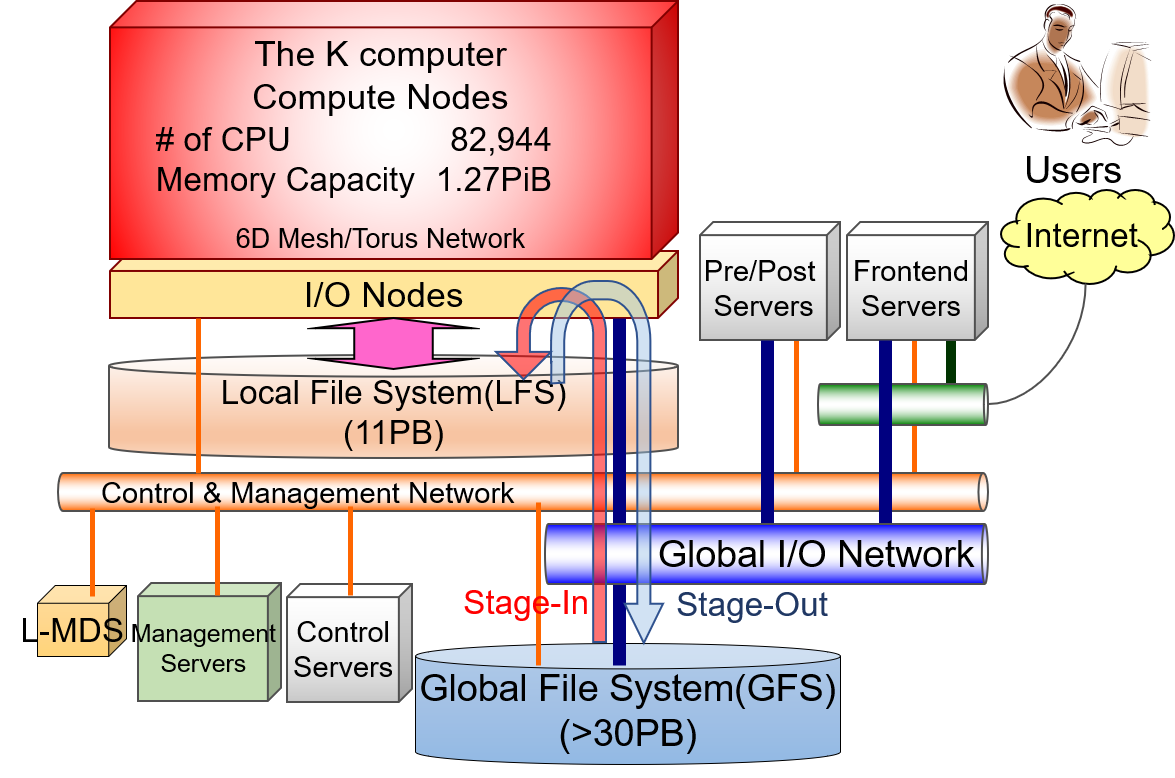
\includegraphics[width=0.6\textwidth]{K-system-overview.png}
\caption{System configuration of the K computer}
\label{fig:K_OVERVIEW}
\end{figure}
%
The LFS was a scratch high-performance storage space which was used during computations,
while the GFS was used to store programs and data with high redundancy.
An enhanced Lustre named Fujitsu Exabyte File System (FEFS)~\cite{fefs:fujitsu-tech-si}
that was based on Lustre version~1.8 was equipped to build both file systems.
The K computer consisted of 82,944 compute nodes and 5,184 I/O nodes,
where every system rack consisted of 96 compute nodes and six I/O nodes.
Every compute node and I/O node were connected through the Tofu interconnect
in a six-dimensional (6D) mesh/torus network represented by $X$, $Y$, $Z$, $A$, $B$, and $C$.
Tofu links of $X$, $Z$, and $B$ were connected in a torus configuration,
while those of $Y$, $A$, and $C$ were connected in a mesh configuration.
However, torus configuration of the $Z$-link was only available in I/O accesses
through I/O nodes because I/O nodes were included in only I/O accesses.
In other cases, the $Z$-link was used in a mesh configuration for
inter-node communications by application jobs.

Figure~\ref{fig:SUBSET_SYSRACK_K} depicts the configuration of a subset of system racks
and I/O accesses from compute nodes towards the LFS.
%
\begin{figure}[tb]
\centering
%% \includegraphics[width=0.7\textwidth]{K-system-rack-config.png}
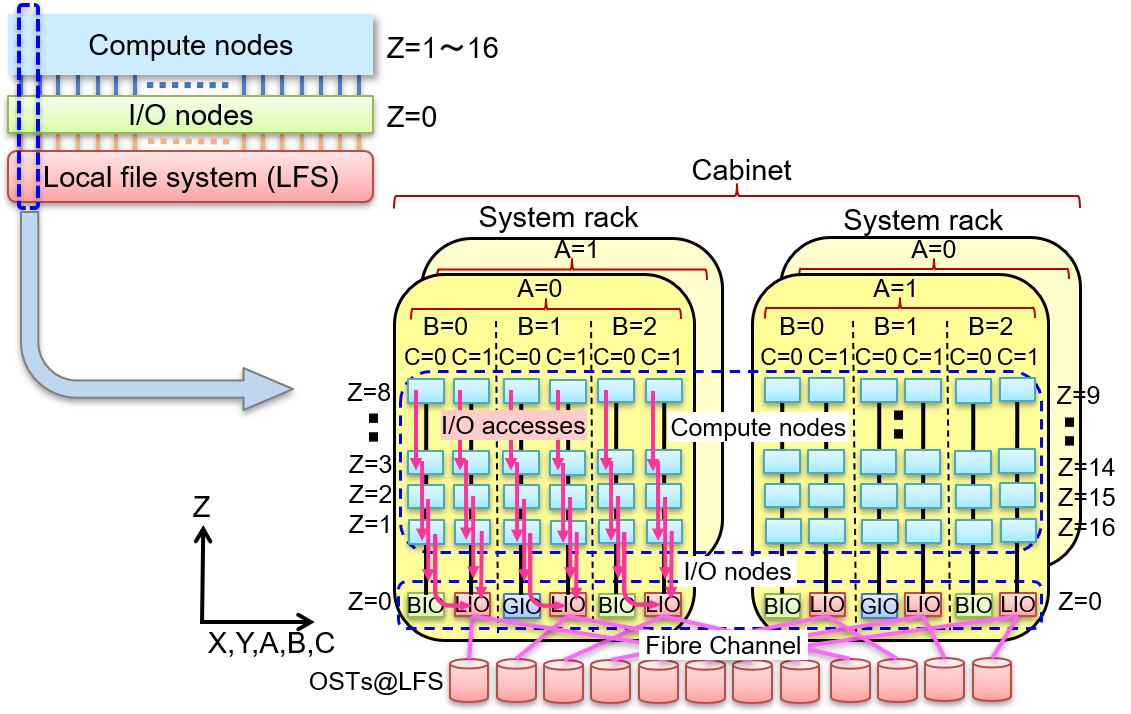
\includegraphics[width=0.8\textwidth]{K-system-rack-config-mod.png}
\caption{Subset of system racks of the K computer and I/O accesses from compute nodes
towards the LFS}
\label{fig:SUBSET_SYSRACK_K}
\end{figure}
%
Each cabinet consists of two system racks, which have two groups separated
by the $A$-link position ($A$=0 and 1) consisting of 48 compute nodes each.
Every compute node was located on $Z$-link positions ranging from $Z$=1 to 8
and from $Z$=9 to 16 in the groups of $A$=0 and 1, respectively,
while I/O nodes were on $Z$=0 in both groups.
Boot-I/O nodes (BIOs) were responsible for system software start-up and
Global I/O nodes (GIOs) were the gateways in accessing the GFS.
The LFS was accessible from compute nodes through OSSes running
on the local-I/O nodes (LIOs).
Every node including I/O nodes consisted of Tofu network router (TNR)~\cite{tofu:micro2012}
where each TNR had 10 communication links
($X+$, $X-$, $Y+$, $Y-$, $Z+$, $Z-$, $A$, $B+$, $B-$, and $C$)
to construct a 6D mesh/torus network.

The number of available OSTs at the LFS was uniquely configured
based on the assigned compute node layout according to
the I/O zoning scheme~\cite{sumimoto:LUG2011}.
I/O zoning scheme was introduced in order to mitigate I/O interference on OSTs
and I/O nodes among jobs by assigning I/O nodes and OSTs on the same $Z$-link
with used compute nodes.
Fig.~\ref{fig:SUBSET_SYSRACK_K} shows I/O accesses from compute nodes
at the system rack in the left side of this figure.
I/O nodes on the same $Z$-links were configured to work with compute nodes
that issued I/O requests, and those I/O nodes
take part in data transfers during I/O accesses on the LFS.
It is noted that I/O paths from compute nodes were automatically routed
to the corresponding I/O nodes (either of BIO, GIO, and LIO) on the same $Z$-link,
then routed to a target OSS running on an LIO.

Performance profiling tools including Tofu~PA addressed to tune performance of
compute nodes and communications among compute nodes.
It is noted that the similar profiling tool is available at
our current HPC system, the supercomputer Fugaku~\cite{fugaku_info:web}
(hereinafter, Fugaku).
%% as remarked  of \cite{fugaku_info:web}.
The tools succeeded to leverage high levels of computing potential of the K computer,
especially in tuning applications utilizing the large number of compute nodes
in terms of data transfer status of each node in addition to CPU and memory utilization.
The only way to tune I/O operations had been benchmark evaluations
because there was not any I/O profiling tool for users to profile activities
of I/O nodes and parallel file systems.
Therefore, it was quite difficult in I/O operation tuning
using only the existing profiling tools.

\subsection{Log collection for monitoring the LFS}
\label{ssec:LOG_COLL_MON}

We have addressed to extract I/O activity information of the LFS
in order to investigate operation status of the LFS
for not only finding malfunctions but also performance tuning.
In this context, we have been conducting to collect log data from servers
associated with the LFS during the K computer operation,
as shown in Figure~\ref{fig:Log-collect-K}.
%
\begin{figure}[tb]
\centering
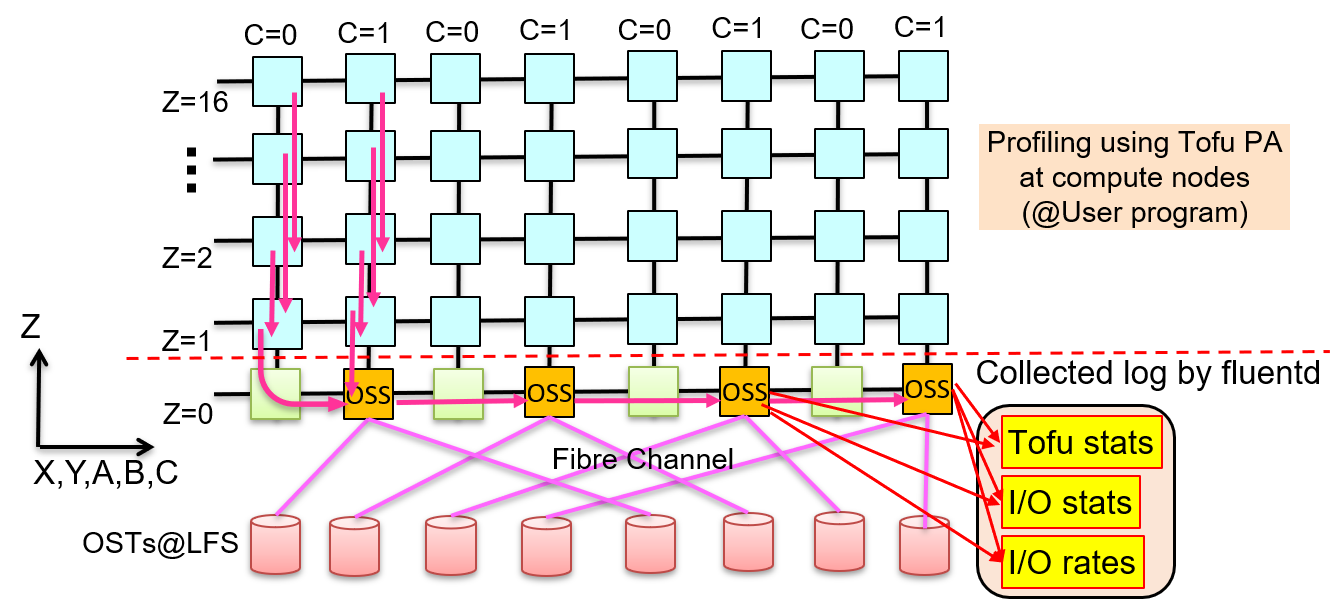
\includegraphics[width=0.72\textwidth]{Log-collect-K-ext.png}
\caption{Log collection from I/O nodes}
\label{fig:Log-collect-K}
\end{figure}
%/
We have deployed {\itshape fluentd} to collect performance metrics associated with
I/O operations from 5,184 I/O nodes including 2,592 LIOs which also acted as OSSes
for the LFS.

% The number of available OSTs at the LFS is uniquely configured based on the shape of
% assigned compute nodes according to the I/O zoning scheme~\cite{sumimoto:LUG2011}.
% I/O zoning scheme has been introduced in order to mitigate I/O interference on OSTs
% and I/O nodes among jobs by assigning I/O nodes and OSTs on the same Z-link
% with used compute nodes.
% All assigned I/O nodes for each job take part in data transfers during I/O accesses on the LFS.
% It is noted that an I/O path from each compute node is automatically routed to an I/O node
% on the same Z-link, then routed to a target OSS on an LIO.

The proposed analysis framework utilized the following three log data collection groups
from large amounts of collected information by {\itshape fluentd}.
%
\begin{itemize}
\item {\tt Tofu stats}: Data transfer status metrics of I/O nodes on each Tofu interconnect link
(the number of transferred packets, amount of transferred data size, and others)
\item {\tt I/O stats}: Statistics of I/O requests obtained from
{\tt /proc/fs/lustre/ost/OSS/ost io/stats} on every OSS
\item {\tt I/O rates}: Amount of size in read and write operations on every OST
\end{itemize}
%
Only the {\tt I/O stats} was collected at one minute intervals,
while the rest were collected at ten minute intervals.
We have selected the ten minute intervals for the I/O-related monitoring as trial
in a conservative manner not to affect I/O node activities for stable production runs
from our empirical study.
We conducted the trial monitoring in the last few months of the K computer operation.
Limited storage space for the I/O related log-collection was another reason
for the ten-minutes intervals.
In the last few months of the K computer operation,
we already collected huge amounts of recorded information
on the log-collection server from other high-priority components
of the K computer for a long time.

The {\tt Tofu stats} consisted of the following packet processing metrics
of the ten Tofu links, which were obtained from the TNR of each I/O node
through the Tofu~PA information in each ten minute interval:
%
\begin{itemize}
\item Cycle counts until target transfer buffer was available in packet transfers
\item Amount of transferred data size
\end{itemize}
%
It is noted that the cycle counts in the {\tt Tofu stats} corresponded to
congestion status since unavailability of transfer buffers in packet processing
closely corresponds to packet transfer congestion.
We conducted to retrieve those metrics from the TNR at every I/O node
during the K computer operation for about a few months
until the end of the K computer operation.

The {\tt I/O stats} consisted of the same statistics with an original Lustre,
where we especially focused on the three statistics,
{\tt req\_qdepth}, {\tt req\_active}, and {\tt req\_waittime}.
These statistics provided the status of I/O requests coming from compute nodes through I/O nodes.
For instance, a large value in both {\tt req\_qdepth} and {\tt req\_waittime} indicated
very busy status of OSSes or idle status of OSSes waiting for the next operation
due to heavy load of an MDS before I/O accesses.
Such situation was not suitable for effective I/O operations.
Since {\tt req\_active} indicated the number of active threads for I/O operations,
high numbers in {\tt req\_active} indicated a very good condition
in terms of I/O accesses.

The {\tt I/O rates} provided I/O throughput status at each OST over time.
Collected I/O throughput information showed I/O behavior on each OST
such as how much I/O bandwidth was achieved in each OST or
how about I/O load balancing was for instance.
Due to the reasons described above, we examined I/O activities
in the two I/O benchmark runs at ten minute intervals as trial,
where each I/O benchmark run took around ten minutes
so that we could observe I/O activities of each I/O benchmark run.
Minimization of monitoring interval time is our future work in Fugaku.

\subsection{Database for executed jobs}
\label{ssec:JOB_DB}

A database to store job information named JOB-DB
was built on a PostgreSQL database server to collect
and refer to job information executed in the K computer.
The JOB-DB kept compute nodes used, compute node layout, elapsed time,
and start and finish times of job execution,
which were associated with a JOB-ID, for instance.
Therefore, we could refer to information about a target job
from the JOB-DB by specifying a JOB-ID.
% We had multiple ways in querying the JOB-DB
% by direct access through a SQL command
% and by indirect access through Redash to retrieve information
% about a target job.

\section{Analysis Framework for I/O Activities}
\label{sec:ANAL_SYS}

As described in Sec.~\ref{ssec:LOG_COLL_MON} and Sec.~\ref{ssec:JOB_DB},
we had monitoring and log collection environment for each component
in the K computer operation.
However, there was not any environment to have holistic I/O activity analysis
for the purpose of investigation and performance tuning.
Considering the complexity in I/O subsystems and I/O software stacks
in a large scale of HPC systems such as the K computer,
we have built an analysis framework in cooperation with
the existing monitoring components described in
Sec.~\ref{ssec:LOG_COLL_MON} and Sec.~\ref{ssec:JOB_DB}.
Since the framework needs to work together with several components
such as the JOB-DB built on a PostgreSQL database and log data
collected by {\itshape fluentd},
we have conducted to build the framework using {\itshape Python}.
Figure~\ref{fig:LOG_ANAL_SYS} depicts an overview of the implemented analysis framework,
which is connected with associated log data collected by {\itshape fluentd}
and the JOB-DB to analyze I/O activities on I/O nodes and the LFS.
%
\begin{figure}[tb]
\centering
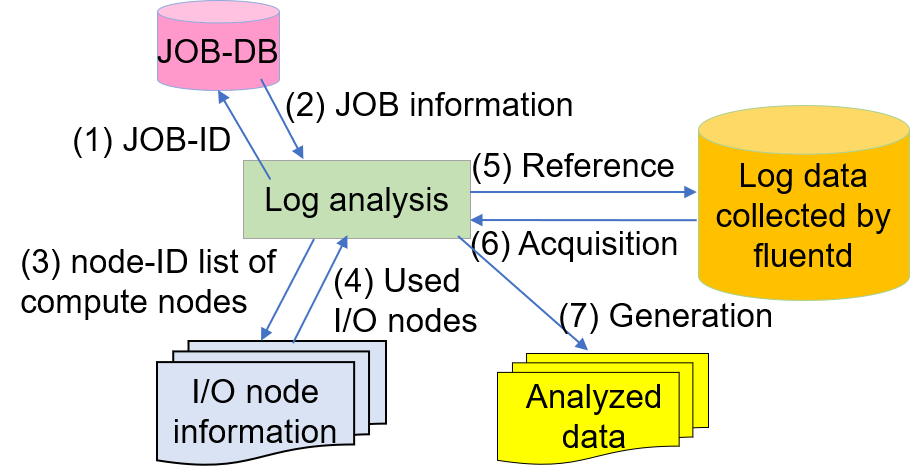
\includegraphics[width=0.6\textwidth]{Log-anal-system.png}
\caption{Functional overview of implemented analysis framework}
\label{fig:LOG_ANAL_SYS}
\end{figure}
%
Given a target JOB-ID, the framework retrieves information of the JOB-ID
such as 6D mesh/torus network positions of used compute nodes and names of
used system racks from the JOB-DB.
Such information about used compute nodes and system racks is utilized
to find used I/O nodes including LIOs from the I/O node table
because the assigned I/O node layout is automatically configured
by the shape of assigned compute nodes.
Besides, start and finish times of the target job obtained from the JOB-DB
are used to pick up essential information associated with the JOB-ID
from a large amount of log data collected by {\itshape fluentd}.

Once the framework collects all essential information, its log analysis function
figures out and gives the following information for the given JOB-ID:
\begin{itemize}
\item Maximum waiting time of each interconnect at each used I/O node ($T_{wait}^{max}$)
from {\tt Tofu stats} log collection
\item Peak bandwidth utilization ratio of the interconnects relative to
the theoretical bandwidth during job execution ($R_{BW}$)
from {\tt Tofu stats} log collection
\item I/O throughput in both write and read operations on each used OST
from {\tt IO rates} log collection
\end{itemize}
%
The former two performance values are calculated by using the packet transfer metrics
obtained from the TNR of used Tofu links, which are obtained from
{\tt Tofu stats} log colection.
The function converts the cycle counts obtained from the TNR
into time values in the unit of second for the $T_{wait}^{max}$.
While the $R_{BW}$ is obtained by dividing the peak bandwidth
in Tofu links of the job with the theoretical bandwidth.
Note that the peak bandwidth is obtained by dividing transferred packet size
with elapsed time of the specified job.
In the proposed framework, we use the $R_{BW}$
to examine effectiveness in packet transfer associated with I/O operations.

While the I/O performance values were obtained by dividing an amount of data size
in read and write operations with a monitoring interval time
(600 seconds in the current configuration) in each snapshot
in order to know I/O throughput at each used OST.
Once the analysis function is executed, data are stored in the CSV format
and associated heat-map image data are stored in the PNG format.

\section{Enhanced MPI-IO Implementation: EARTH on K}
\label{sec:EARTH}

In order to examine effectiveness of the proposed framework,
we have conducted to evaluate MPI-IO benchmark runs.
In this context, we have picked up our enhanced MPI-IO implementations
in addition to the original MPI-IO implementation at the K computer.

MPI-IO is an I/O interface including parallel I/O in the MPI standard~\cite{mpi-forum:web}.
An MPI library for the K computer supports MPI-IO functions for the FEFS
using MPI-IO implementation named ROMIO~\cite{thakur:romio}.
Two-phase I/O optimization in ROMIO
improves collective MPI-IO performance in accessing
non-contiguous data layouts in each process by rearrangement
to form large data access space as much as possible in each process
performing I/O (aggregator).
Although two-phase I/O optimization of ROMIO improves collective MPI-IO performance,
the implementation on the K computer uses an old implementation of ROMIO
which is not optimized for Lustre.
Therefore, the original MPI-IO implementation is not suitable
for the FEFS to achieve high I/O performance.

The current ROMIO with the improved two-phase I/O for Lustre~\cite{lustre-adio:whpaper-2008}
has a potential to improve performance on the FEFS.
Our enhanced MPI-IO implementation named ``EARTH on K''
(hereinafter, EARTH) has been developed for the K computer
based on the improved two-phase I/O with topology-aware performance optimizations
for collective MPI-IO at the FEFS.
We have already reported performance improvements by using the EARTH
in some conference papers~\cite{tsujita:WS_EuroMPI2014,tsujita:hpcasia18},
there is not any evidences what kind of improvements has been achieved
in underlying interconnects among I/O nodes or OST activities.
In this context, we have investigated some advanced functions of
this implementation with the proposed framework.

Compared with the original MPI-IO, EARTH has advanced optimizations
controlled by the following three parameters represented by {\tt agg}, {\tt req},
and {\tt rr}, respectively:
%
\begin{itemize}
\item {\tt agg}: Striping-aware aggregator layout
\item {\tt req}: I/O throttling and associated stepwise data aggregation
with a given number of I/O requests per step
\item {\tt rr}: Round-robin aggregator layout among compute nodes
\end{itemize}
%

ROMIO deploys one aggregator in each compute node, and its layout is dependent on
MPI rank layout among compute nodes.
In HPC systems, users have been focusing on MPI rank layout
for communication performance among compute nodes.
However, such optimizations are not always suited for aggregator layout
with respect to interconnects among compute nodes and I/O nodes
or layout of OSSes/OSTs of a Lustre file system.
In such layout, contention in data transfer happens
on network paths among compute nodes and a Lustre file system.

The striping-aware aggregator layout mitigates data transfer congestion
by suitable aggregator layout.
Figure~\ref{fig:AGG_STR_AWARE} shows aggregator layouts with and
without striping awareness in accessing four OSTs by 16 aggregators,
where numbers in circles represent MPI ranks
and the numbers ranging from {\itshape i} to {\itshape iv} represent
the order of striping accesses.
%
\begin{figure}[htb]
\centering
\begin{minipage}[t]{0.42\textwidth}
\centering
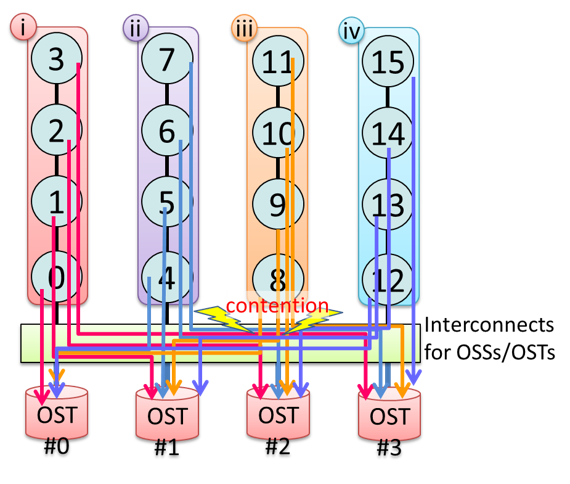
\includegraphics[width=0.96\textwidth]{MPI-IO-non-agg-opt.png}
\subcaption{Without striping-awareness}
\label{fig:WO_STR_AWARE}
\end{minipage}
\noindent
\begin{minipage}[t]{0.42\textwidth}
\centering
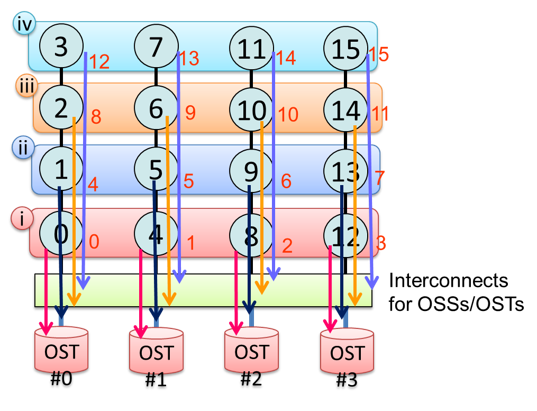
\includegraphics[width=0.96\textwidth]{MPI-IO-with-agg-opt.png}
\subcaption{With striping-awareness}
\label{fig:WITH_STR_AWARE}
\end{minipage}
\caption{Aggregator layouts with and without striping awareness}
\label{fig:AGG_STR_AWARE}
\end{figure}
%
By placing aggregators in an MPI rank order
as shown in Fig.~\ref{fig:WO_STR_AWARE},
we may face contention in a path towards target OSTs.
On the other hand, a striping-aware layout shown in
Fig.~\ref{fig:WITH_STR_AWARE},
renumbering the order of aggregators in the red-colored numbers,
eliminates data transfer congestion on every I/O path
because I/O flows of every I/O path towards a target OST are
evenly distributed for a striping access pattern against OSTs.

Figure~\ref{fig:IO_THROT} illustrates
I/O throttling scheme operated by 192 aggregators accessing 12 OSTs,
where we assume every process acts as an aggregator.
%
\begin{figure}[htb]
\centering
\begin{minipage}[b]{0.45\textwidth}
\centering
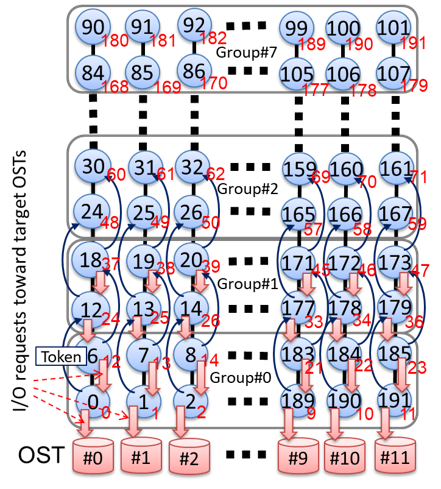
\includegraphics[width=0.98\textwidth]{MPI-IO-throttling.png}
\subcaption{I/O throttling with token relay}
\label{fig:IO_THROT}
\end{minipage}
\noindent
\begin{minipage}[b]{0.45\textwidth}
\centering
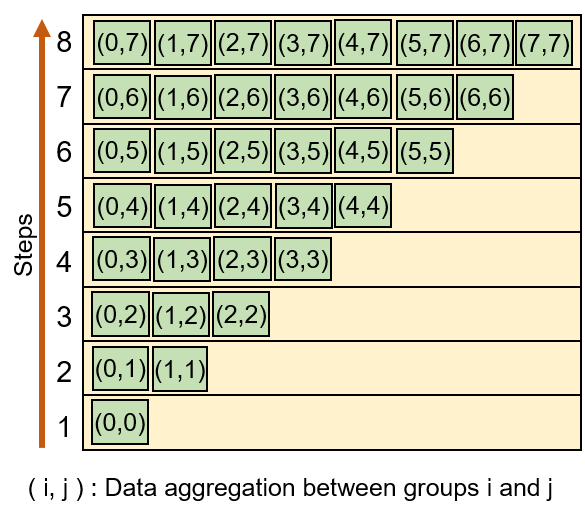
\includegraphics[width=0.96\textwidth]{data_agg_step_wise.png}
\subcaption{Stepwise data aggregation}
\label{fig:STEP_WISE_AGG}
\end{minipage}
\caption{I/O request throttling with stepwise data aggregation}
\label{fig:IO_THROT_DATA_AGG}
\end{figure}
%
Numbers in circles represent MPI ranks, and red-colored numbers neighboring
to the circles are the aggregator layout orders configured by
the striping-aware aggregator layout.
Two-phase I/O consists of repetitive operations of
data aggregation on every aggregator and I/O accesses by aggregators.
We may have I/O request contention on OSTs
if we have I/O accesses simultaneously from all aggregators.
The I/O throttling scheme shown in this figure alleviates I/O request contention
on OSTs by issuing I/O requests from aggregators in each group in a stepwise manner
from the younger number group by relaying tokens from an aggregator that finishes
I/O accesses to a corresponding aggregator in the next group.
The number of groups can be tuned at runtime through {\tt MPI\_Info\_set()}
or an environment variable.
It is also noted that EARTH also supports I/O request throttling
even if we disable two-phase I/O in collective MPI-IO.

Stepwise data aggregation shown in
Fig.~\ref{fig:STEP_WISE_AGG}
is another optimization associated with the I/O throttling.
Compared with simultaneous data aggregation by all the processes,
we can eliminate congestion in data transfers among compute nodes
by stepwise data aggregations issued from younger number group.
In this figure, we represent data aggregation between
the groups numbered by $i$ and $j$ as $(i,j)$,
which is equivalent to $(j,i)$.
In the first step (step=1), processes in the first group numbered as 0
initiates data transfers to aggregators on every group
numbered from 0 to 7, described by $(0,k)$, where $k=0\mathchar`-7$.
However, in the first step, only the $(0,0)$ is carried out
because other groups are not ready in data aggregation.
In the next step (step=2), the second group numbered as 1 initiates
data aggregation of $(1,k)$, where $k=0\mathchar`-7$,
and only data aggregations of $(0,1)$, which is equivalent to $(1,0)$,
and $(1,1)$ complete in this step.
Finally in the last step (step=8), the last group numbered as 7
initiates data aggregations of $(7,k)$, where $k=0\mathchar`-7$.
Then the remaining aggregations denoted by $(k,7)$,
where $k=0\mathchar`-7$, complete in this step.

Figure~\ref{fig:AGG_RR_LAYOUT} shows examples of blocked and round-robin
aggregator layouts, where we have eight aggregators from 16 processes
deployed among four compute nodes in a blocked layout.
%
\begin{figure}[tb]
\centering
\begin{minipage}[t]{0.36\textwidth}
\centering
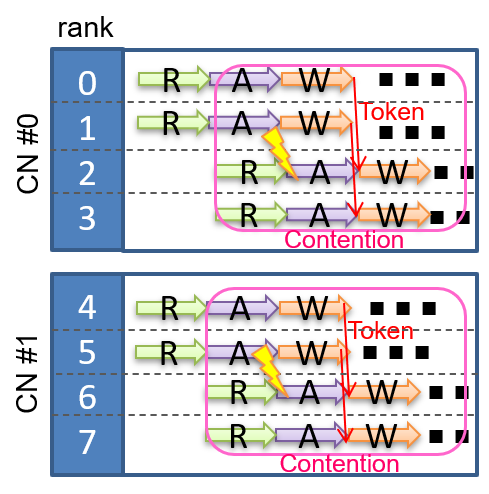
\includegraphics[width=0.96\textwidth]{MPI-IO-agg-block_layout.png}
\subcaption{Blocked layout}
\label{fig:BLK_LAYOUT}
\end{minipage}
\noindent
\begin{minipage}[t]{0.36\textwidth}
\centering
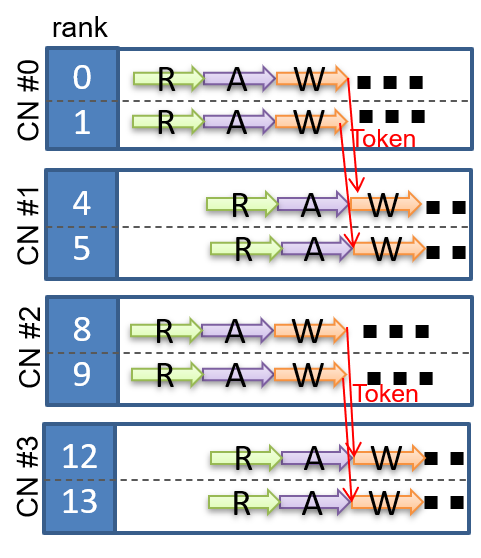
\includegraphics[width=0.96\textwidth]{MPI-IO-agg-rr_layout.png}
\subcaption{Round-robin layout}
\label{fig:RR_LAYOUT}
\end{minipage}
\caption{Aggregator layouts with blocked and round-robin manners,
utilizing I/O throttling and step-wise data aggregation in write operations}
\label{fig:AGG_RR_LAYOUT}
\end{figure}
%
Horizontal colored arrows represented by {\itshape R}, {\itshape A},
and {\itshape W} stand for
read, data aggregation, and write phases in two-phase I/O during collective write
operations, respectively.
As shown in this figure, I/O throttling scheme relays tokens among aggregators.
When we have a blocked aggregator layout as shown in
Fig.~\ref{fig:BLK_LAYOUT},
four processes in the two compute nodes ({\itshape CN\,\#0} and {\itshape CN\,\#1})
work as aggregators, which are from 0 to 7 in MPI ranks.
As a result, we may have contention within the same compute node
to proceed each phase of two-phase I/O.
It is also noted that such layout leads to high I/O workload
in each node compared with other compute nodes without aggregators.
Meanwhile, the round-robin aggregator layout in
Fig.~\ref{fig:RR_LAYOUT}
can distribute I/O workload evenly
among compute nodes, and this layout also prevents aggregators
from I/O access contention within the same compute node
by reducing the number of aggregators in the same compute node.
%% if we have multiple aggregators on a subset of compute nodes.

Although the above enhancements outperformed the original version
in an empirical study using I/O benchmark runs~\cite{tsujita:WS_EuroMPI2014,tsujita:hpcasia18},
there was not any investigations about performance impact
of those optimizations in I/O nodes or underlying file systems.
One of the main reasons is the lack of tools to characterize optimization
effects in data transfers among I/O nodes and I/O accesses
against the LFS at the K computer.
By using the proposed framework, we examined their advanced features
at the K computer in the following section.

\section{Experimental Evaluation}
\label{sec:EVAL}

We conducted to examine functionalities of the proposed framework
at the K computer through two I/O benchmark runs,
IOR~\cite{IOR:web} and HPIO~\cite{ching:ipdps06},
about the original MPI-IO implementation and EARTH.
Although the K computer was already dismantled,
we believe that results and experiences obtained from the evaluations
provide useful hints for current HPC systems including Fugaku.
Although IOR supports two file creation modes, accessing
file per rank and shared access to a single file,
we utilized the shared access mode with collective MPI-IO.
Meanwhile, HPIO supports I/O accesses for non-contiguous data layout,
and we executed collective MPI-IO for the data layout.
For both benchmark runs, we initiated 12,288 processes on 3,072 compute nodes
forming a logical 3D layout of $8\times12\times32$ in order to eliminate I/O interference
from other jobs. According to the 3D layout of assigned compute nodes,
192 OSTs were assigned for parallel I/O, and we set 192 as a stripe count
to use all available OSTs.
We set 256~MiB and 64~MiB in stripe size in the IOR run and the HPIO run, respectively.

In both benchmark runs, every processes worked as aggregators
with ascending order layout in MPI ranks from zero in the original MPI-IO
under default configuration.
On the one hand, 6,144 processes were chosen to be aggregators in the EARTH case
in order to examine performance impact of aggregator layout among compute nodes
according to optimization configuration of the EARTH.
In this paper, {\tt original} stands for the original MPI-IO,
while a combination of the three optimization parameters,
{\tt agg}, {\tt rr}, and {\tt req}, indicates MPI-IO of the EARTH.
Concerning the EARTH use case, {\tt agg=1} stands for striping-aware aggregator layout
and {\tt rr=1} denotes round-robin aggregator layout among compute nodes.
A zero value in each case stands for deactivation in the corresponding layout optimization.
The last parameter {\tt req} with a number describes the number of I/O requests
going to each OST per step in I/O throttling and stepwise data aggregation
except that {\tt req=0} denotes deactivation of I/O throttling and stepwise aggregation.

In the IOR benchmark run, we conducted collective MPI-IO without two-phase I/O.
In this paper, we describe collective MPI-IO with and without two-phase I/O
by giving ``T:'' and ``N:'' at the beginning of the parameter configuration notation
such as {\tt T:original} and {\tt N:original}, respectively.

\subsection{Benchmark configuration}

We conducted to evaluate collective MPI-IO in the two benchmark runs, IOR and HPIO
with the proposed framework.
In both cases, we enabled two-phase I/O implemented in ROMIO.

\subsubsection{IOR}

The following command was executed in write operations to generate
a shared file of 3~TiB (= 256~MiB $\times$ 12,288) per iteration:
%
\begin{verbatim}
$ ior -i 5 -a MPIIO -c -U hints_info -k -m -vvv -w -t 256m -b 256m \
    -o ${TARGET_DIR}/test-IOR.dat -d 0.1
\end{verbatim}
%
We executed read operations with the same command changing ``-w'' by ``-r'',
followed by write operations with the above command
in every optimization parameter configuration.
``{\tt hints\_info}'', is a file describing some hints associated with
I/O operations such as the number of processes per node and so forth.
%
% \begin{figure}[tb]
% \begin{verbatim}
%        IOR_HINT__MPI__romio_lustre_co_ratio=32
%        IOR_HINT__MPI__cb_config_list=*:4
%        IOR_HINT__MPI__romio_cb_read=enable
%        IOR_HINT__MPI__romio_cb_write=enable
% \end{verbatim}
% \caption{Hints passed to the IOR benchmark code}
% \label{fig:IOR_HINTS}
% \end{figure}
%
A target file ({\tt test-IOR.dat}) was generated in the directory
({\tt \$\{TARGET\_DIR\}}) with 192 stripe count.
We carried out collective MPI-IO with and without two-phase I/O by enabling
or disabling ``{\tt romio\_cb\_write}'' and ``{\tt romio\_cb\_read}''
through the ``{\tt hints\_info}.''
%

\subsubsection{HPIO}

We executed the following command for write operations to generate
a shared file of about 2.1~TiB ($\approx$ (5,992~B + 256~B) $\times$ 12,288 $\times$ 30,729 - 256~B)
per iteration, followed by read operations in non-contiguous access pattern
on a target file with specifying the number of processes per node ({\tt -H cb\_config\_list=*:4}) and parameter to tune the number of aggregators to be
6,144 (=$192 \times 32$):
%
\begin{verbatim}
$ hpio -n 12288 -n 0010 -r 6 -B -s 5992 -c 30729 -p 256 -m 01 -O 11 -f 0 \
  -S 0 -a 0 -g 2 -H cb_config_list=*:4 -H romio_lustre_co_ratio=32 \
  -d ${TARGET_DIR} -w 1
\end{verbatim}
%
Note that the option, ``{\tt cb\_config\_list}'' was available only for
the EARTH case, and thus all processes worked as aggregators
in the original case as we explained.
The target file was generated in the directory {\tt \$\{TARGET\_DIR\}}
with 192 stripe count. We carried out the collective MPI-IO
only with two-phase I/O because collective MPI-IO without two-phase I/O was
time-consuming under the non-contiguous access pattern and
it was difficult to do in a limited machine time.

\subsection{Benchmark results}

Figure~\ref{fig:IOR_HPIO_PERF} shows averaged I/O throughput values
with standard deviations for the IOR and HPIO benchmarks. 
%
\begin{figure}[tb]
\centering
\begin{minipage}[t]{0.46\textwidth}
 \centering
 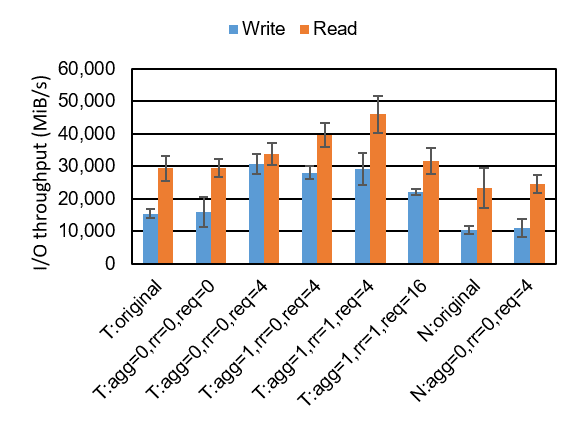
\includegraphics[width=1.0\textwidth]{IOR-results-ext.png}
 \subcaption{IOR benchmark}
 \label{fig:IOR_PERF}
\end{minipage}
%
\noindent
\begin{minipage}[t]{0.46\textwidth}
 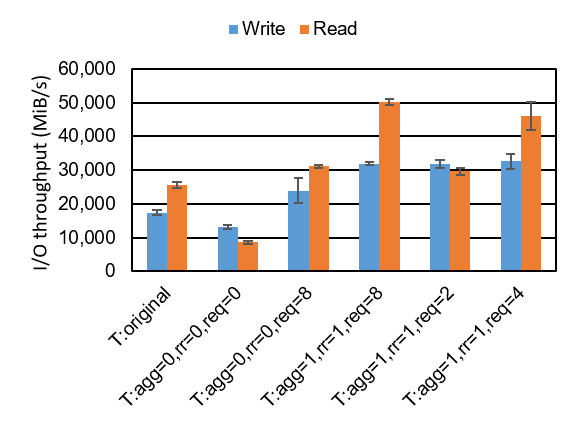
\includegraphics[width=1.0\textwidth]{hpio-results-ext.png}
 \subcaption{HPIO benchmark}
 \label{fig:HPIO_PERF}
\end{minipage}
\caption{
Benchmark results of the original MPI-IO and EARTH with several optimization
configurations by using (a) IOR and (b) HPIO}
\label{fig:IOR_HPIO_PERF}
\end{figure}
%

The original MPI-IO operations with and without two-phase I/O represented by
{\tt T:original} and {\tt N:original} showed poor performance in both read and write
operations in the IOR runs.
The same situation was observed for the {\tt T:original} case in the HPIO runs.
EARTH with full optimization in aggregator layout, I/O request throttling,
and stepwise data aggregation outperformed other cases by setting four requests per step
({\tt T:agg=1,rr=1,req=4}) in the IOR runs and eight requests per step
({\tt T:agg=1,rr=1,req=8}) in the HPIO runs.
However, performance was degraded by changing the number of requests per step
or deactivating aggregator layout optimization.
In addition, the EARTH case using only I/O throttling without two-phase I/O
({\tt N:agg=0,rr=0,req=4}) could not improve I/O performance
compared to the original case ({\tt N:original}) in the IOR runs.

Although we learned optimization effects through such empirical benchmark runs
in our previous research papers~\cite{tsujita:WS_EuroMPI2014,tsujita:hpcasia18},
it was not clear about the performance impact of the optimization configuration
on I/O nodes, Tofu links among I/O nodes, and the LFS.
We report investigations of each component using the proposed framework
in the following subsections.

% \subsection{Analysis of OSS stats}
% \subsection{Analysis of {\tt I/O stats}}
\subsection{I/O request status at file system servers}

Figure~\ref{fig:IOR_OST_IO_STATS} shows the mean values of
{\tt req\_qdepth}, {\tt req\_waittime}, and {\tt req\_active}
from {\tt I/O stats} log collection during I/O operations
at the IOR benchmark run.
%
\begin{figure}[tb]
\centering
\begin{minipage}[t]{0.46\textwidth}
 \centering
 %%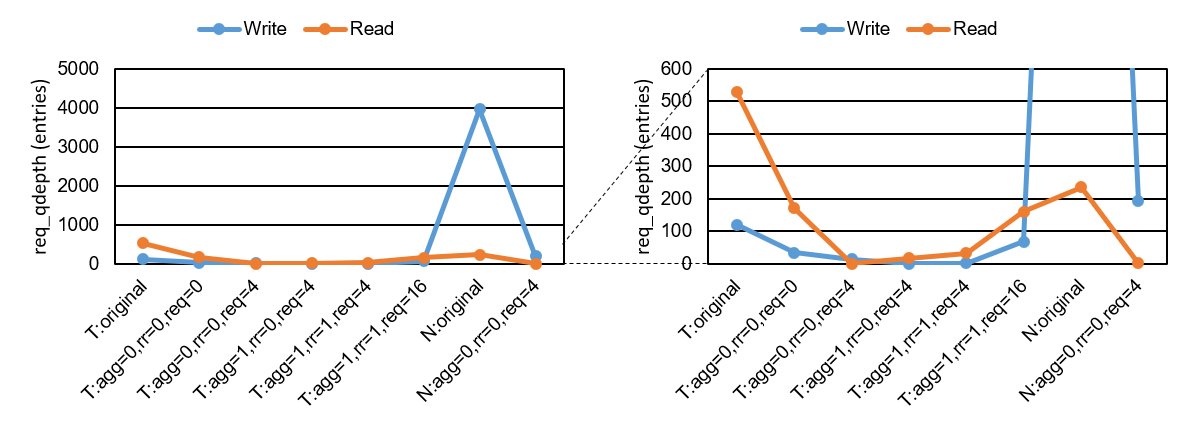
\includegraphics[width=1.0\textwidth]{IOR-ost_io_stats-qdepth-ext-dual.png}
 %%\subcaption{{\tt req\_qdepth} (Left: Overall, Right: Zoomed less than or equal to 600 entries)}
 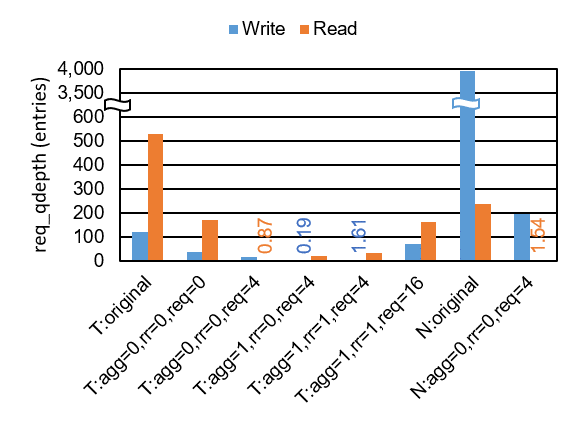
\includegraphics[width=0.96\textwidth]{IOR-ost_io_stats-qdepth-ext.png}
 \subcaption{{\tt req\_qdepth}: The vertical axis is expanded from 600 to 3,500}
 \label{fig:IOR_req_qdepth}
\end{minipage}
%
%\noindent
\begin{minipage}[t]{0.46\textwidth}
 \centering
 %%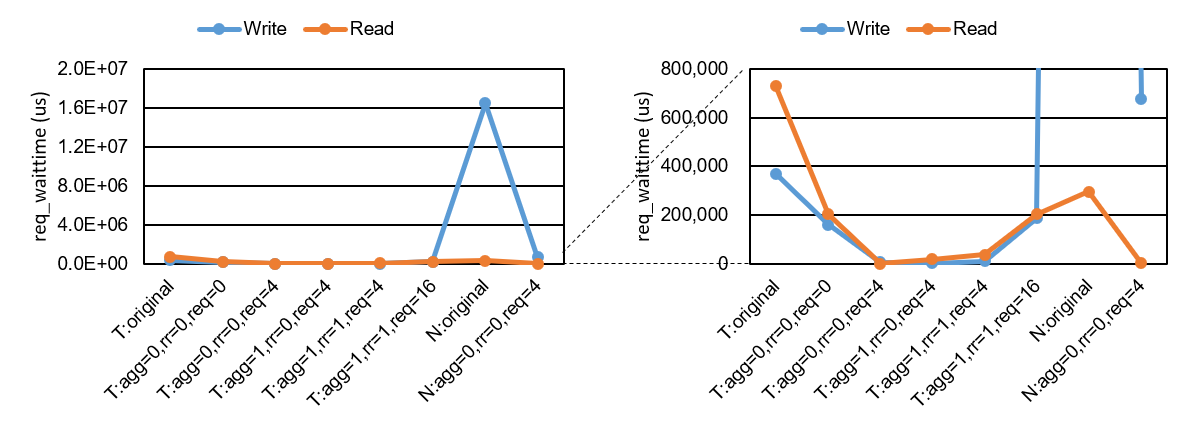
\includegraphics[width=1.0\textwidth]{IOR-ost_io_stats-waittime-ext-dual.png}
 %%\subcaption{{\tt req\_waittime} (Left: Overall, Right: Zoomed less than or equal to 800\,ms)}
 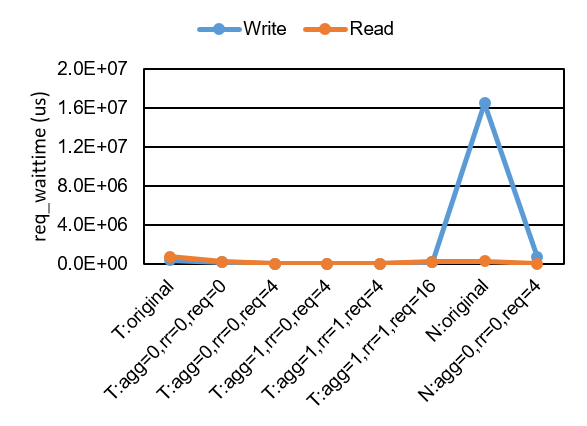
\includegraphics[width=0.96\textwidth]{IOR-ost_io_stats-waittime-ext.png}
 \subcaption{{\tt req\_waittime}: The vertical axis is expanded from 800\,ms to 16\,s}
 \label{fig:IOR_req_waittime}
\end{minipage}
%
\noindent
\begin{minipage}[t]{0.44\textwidth}
 \centering
 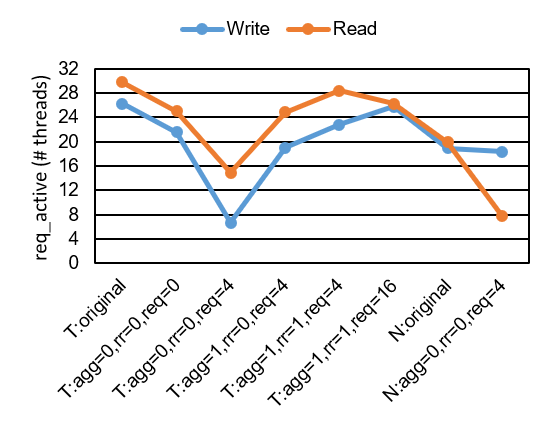
\includegraphics[width=1.0\textwidth]{IOR-ost_io_stats-active-ext.png}
 \subcaption{{\tt req\_active}}
 \label{fig:IOR_req_active}
\end{minipage}
%
\caption{Mean stats values obtained from OSSes using our analysis framework
during the IOR benchmark run, where numbers represent very small values}
\label{fig:IOR_OST_IO_STATS}
\end{figure}
%
As shown in Fig.~\ref{fig:IOR_req_qdepth}, the two original cases
with or without two-phase I/O, {\tt T:original} and {\tt N:original},
had the largest number of requests in a request queue
in each I/O operations with or without two-phase I/O.
Fig.~\ref{fig:IOR_req_waittime} shows that those cases also took
the longest time to proceed requests
in each I/O operations with or without two-phase I/O.
Additionally, Fig.~\ref{fig:IOR_req_active} shows
the highest number of I/O threads in the original case
with two-phase I/O.
Note that the maximum number of threads at each OSS of the LFS was 32
at the K computer.
Through these results, we determined that the two original cases,
{\tt T:original} and {\tt N:original}, were not suited for
I/O request processing at OSSes.

While the EARTH use case with good I/O performance ({\tt T:agg=1,rr=1,req=4})
showed small number of requests in the queue,
as shown in Fig.~\ref{fig:IOR_req_qdepth}.
Fig.~\ref{fig:IOR_req_waittime} also shows
the fact that this case took quite short times to process I/O requests.
Additionally, Fig.~\ref{fig:IOR_req_active} shows
many I/O threads were active in this case.

Figure~\ref{fig:HPIO_OST_IO_STATS} shows the same statistics obtained
in the HPIO benchmark run.
%
\begin{figure}[tb]
\centering
\begin{minipage}[t]{0.44\textwidth}
 \centering
 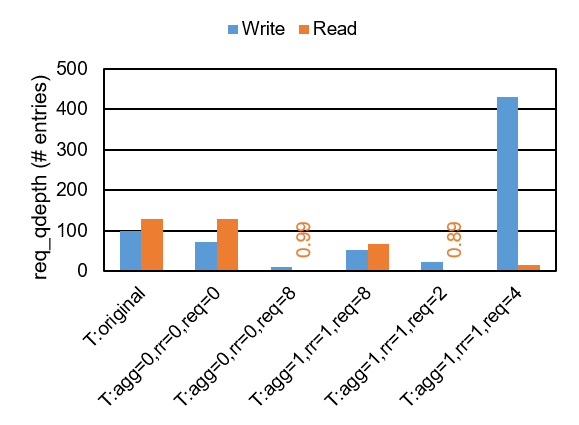
\includegraphics[width=1.0\textwidth]{hpio-ost_io_stats-qdepth-ext.png}
 \subcaption{{\tt req\_qdepth}}
 \label{fig:HPIO_req_qdepth}
\end{minipage}
%
\noindent
\begin{minipage}[t]{0.44\textwidth}
 \centering
 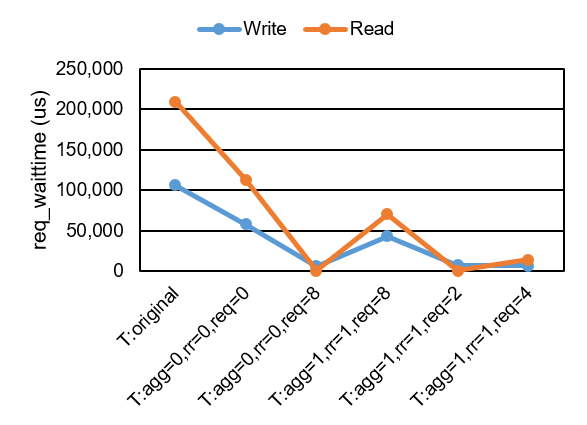
\includegraphics[width=1.0\textwidth]{hpio-ost_io_stats-waittime-ext.png}
 \subcaption{{\tt req\_waittime}}
 \label{fig:HPIO_req_waittime}
\end{minipage}
%
\noindent
\begin{minipage}[t]{0.44\textwidth}
 \centering
 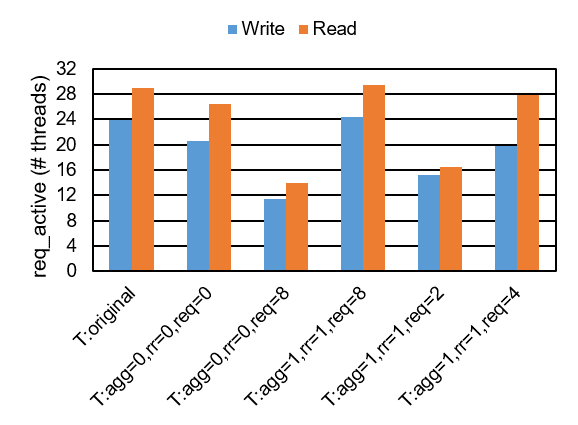
\includegraphics[width=1.0\textwidth]{hpio-ost_io_stats-active-ext.png}
 \subcaption{{\tt req\_active}}
 \label{fig:HPIO_req_active}
\end{minipage}
%
\caption{Mean stats values obtained from OSSes using our analysis framework
during the HPIO benchmark run, where numbers represent very small values}
\label{fig:HPIO_OST_IO_STATS}
\end{figure}
%
Similar to the IOR run, the original use case was not good compared
with the EARTH use case with good optimization configuration
indicated by {\tt T:agg=1,rr=1,req=8}.

\subsection{Bandwidth utilization and waiting times in data transfers on Tofu interconnects of I/O nodes}

Figure~\ref{fig:IOR_ION_TOFU_BWU_WAIT_TIME} shows mean values of
(a) $R_{BW}$ and (b) $T_{wait}^{max}$ on Tofu links of I/O nodes used.
%
\begin{figure}[tb]
\centering
\begin{minipage}[t]{0.48\textwidth}
 \centering
 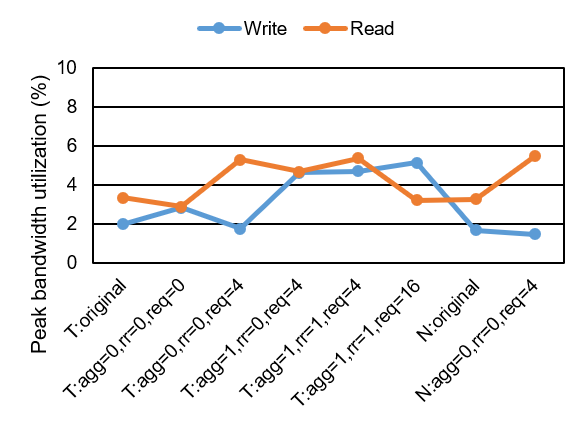
\includegraphics[width=1.0\textwidth]{IOR-bwu-IO-nodes-ext.png}
 \subcaption{$R_{BW}$}
 \label{fig:IOR_ION_TOFU_BW_UTIL}
\end{minipage}
%
\noindent
\begin{minipage}[t]{0.48\textwidth}
 \centering
 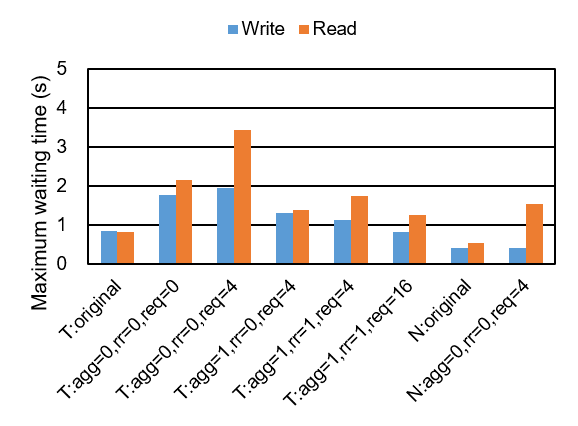
\includegraphics[width=1.0\textwidth]{IOR-zero_credit_sec-IO-nodes-ext.png}
 \subcaption{$T_{wait}^{max}$}
 \label{fig:IOR_ION_TOFU_WAIT_TIME}
\end{minipage}
\caption{
Mean values for (a) $R_{BW}$ and (b) $T_{wait}^{max}$ on the Tofu interconnects
among I/O nodes used during the IOR benchmark run}
\label{fig:IOR_ION_TOFU_BWU_WAIT_TIME}
\end{figure}
%
Concerning bandwidth utilization shown in
Fig.~\ref{fig:IOR_ION_TOFU_BW_UTIL},
the original MPI-IO use case showed the lowest utilization,
while the full set of EARTH optimizations such as {\tt T:agg=1,rr=1,req=4}
led to higher levels of bandwidth utilization relative to other cases.
While the use cases without two-phase I/O,
{\tt N:original} and {\tt N:agg=0,rr=0,req=4}, showed
larger number of requests in queue, especially in write operations.
By considering effectiveness in data transfers among I/O nodes via Tofu interconnects,
a higher utilization was preferable.
Within this context, the above optimized case was suitable for I/O optimization.

Fig.~\ref{fig:IOR_ION_TOFU_WAIT_TIME}
shows that the enhanced implementation
without aggregator layout optimization indicated by {\tt T:agg=0,rr=0,req=4}
took the longest times.
It is also noted that this case also performed the lowest bandwidth utilization
in write operations,
as shown in Fig.~\ref{fig:IOR_ION_TOFU_BW_UTIL}.
It is notable that the lack of aggregator layout optimization in the EARTH case
led to a negative impact in data transfers on Tofu interconnects among I/O nodes.

In a similar way, Fig.~\ref{fig:HPIO_ION_TOFU_BWU_WAIT_TIME} shows
bandwidth utilization ratios and waiting times in data transfers
on Tofu links of I/O nodes used at the HPIO benchmark run.
%
\begin{figure}[tb]
\centering
\begin{minipage}[t]{0.48\textwidth}
 \centering
 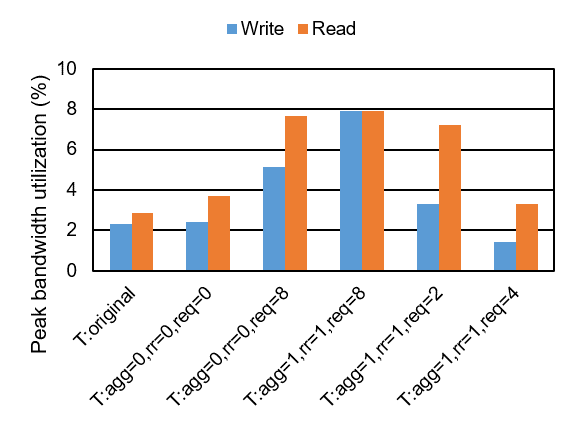
\includegraphics[width=0.98\textwidth]{hpio-bwu-IO-nodes-ext.png}
 \subcaption{$R_{BW}$}
 \label{fig:HPIO_ION_TOFU_BW_UTIL}
\end{minipage}
%
\noindent
\begin{minipage}[t]{0.48\textwidth}
 \centering
 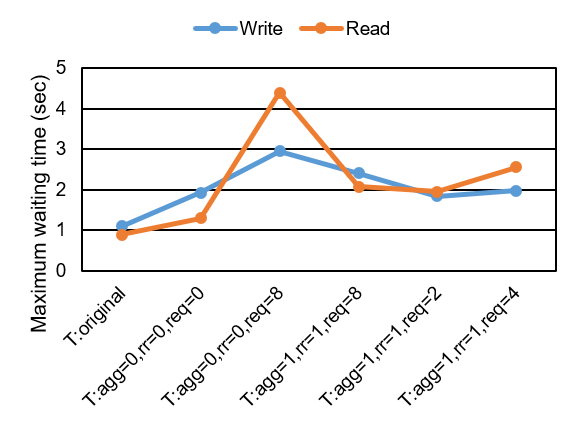
\includegraphics[width=0.98\textwidth]{hpio-zero_credit_sec-IO-nodes-ext.png}
 \subcaption{$T_{wait}^{max}$}
 \label{fig:HPIO_ION_TOFU_WAIT_TIME}
\end{minipage}
\caption{Mean values for (a) $R_{BW}$ and (b) $T_{wait}^{max}$ on the Tofu interconnects
among I/O nodes used during the HPIO benchmark run}
\label{fig:HPIO_ION_TOFU_BWU_WAIT_TIME}
\end{figure}
%
The EARTH use case with the best configuration ({\tt T:agg=1,rr=1,req=8}) also
outperformed other cases in
Fig.~\ref{fig:HPIO_ION_TOFU_BW_UTIL}.
This case also minimized waiting times in both read and write operations
among the EARTH use cases in Fig.~\ref{fig:HPIO_ION_TOFU_WAIT_TIME}.

\subsection{Load balancing in I/O throughput at OSTs}

Figure~\ref{fig:IOR_OST_BW_HMAP_WR} shows write throughput heat-maps
ranging from 0 to 160\,MiB/s
among the 192 OSTs used during the IOR benchmark runs.
%
\begin{figure}[tb]
%% \centering
\begin{minipage}[t]{0.06\textwidth}
 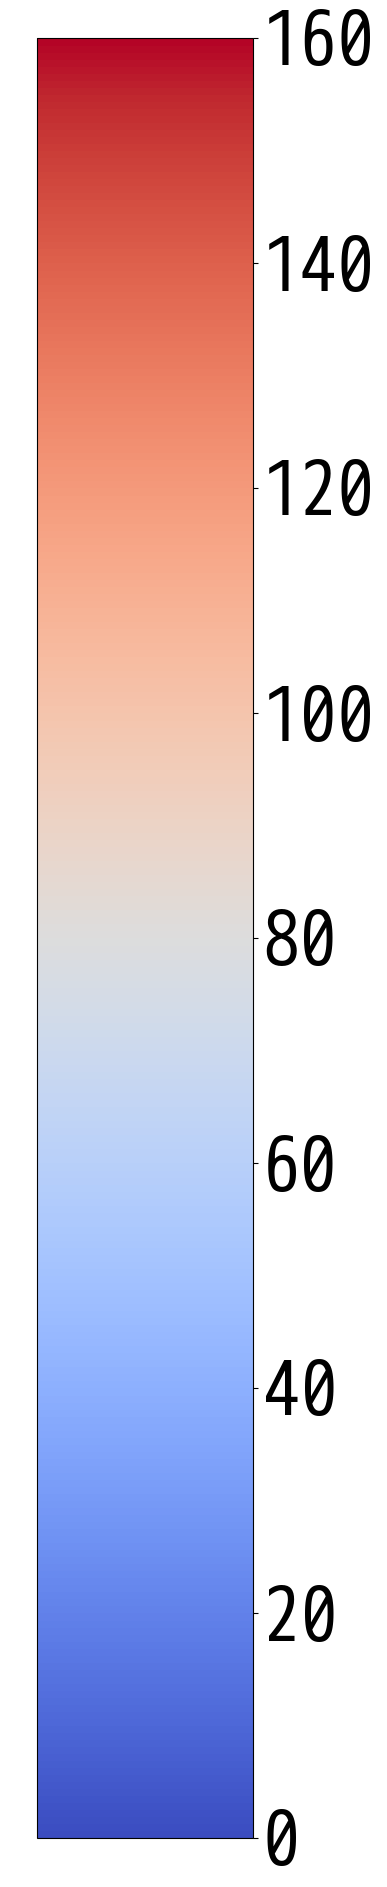
\includegraphics[width=0.98\textwidth,height=0.14\textheight]{hmap-colorbar-mod2.png}
\end{minipage}
%
\noindent
\begin{minipage}[t]{0.3\textwidth}
 \centering
 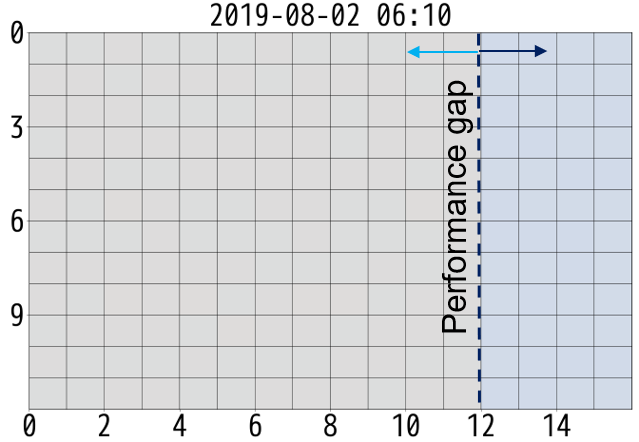
\includegraphics[width=0.98\textwidth]{IOR-OST_bw_hmap-TP-orig-write-mod.png}
 \subcaption{{\tt T:original}}
 \label{fig:IOR_OST_WR_ORIG}
\end{minipage}
%
\noindent
\begin{minipage}[t]{0.3\textwidth}
 \centering
 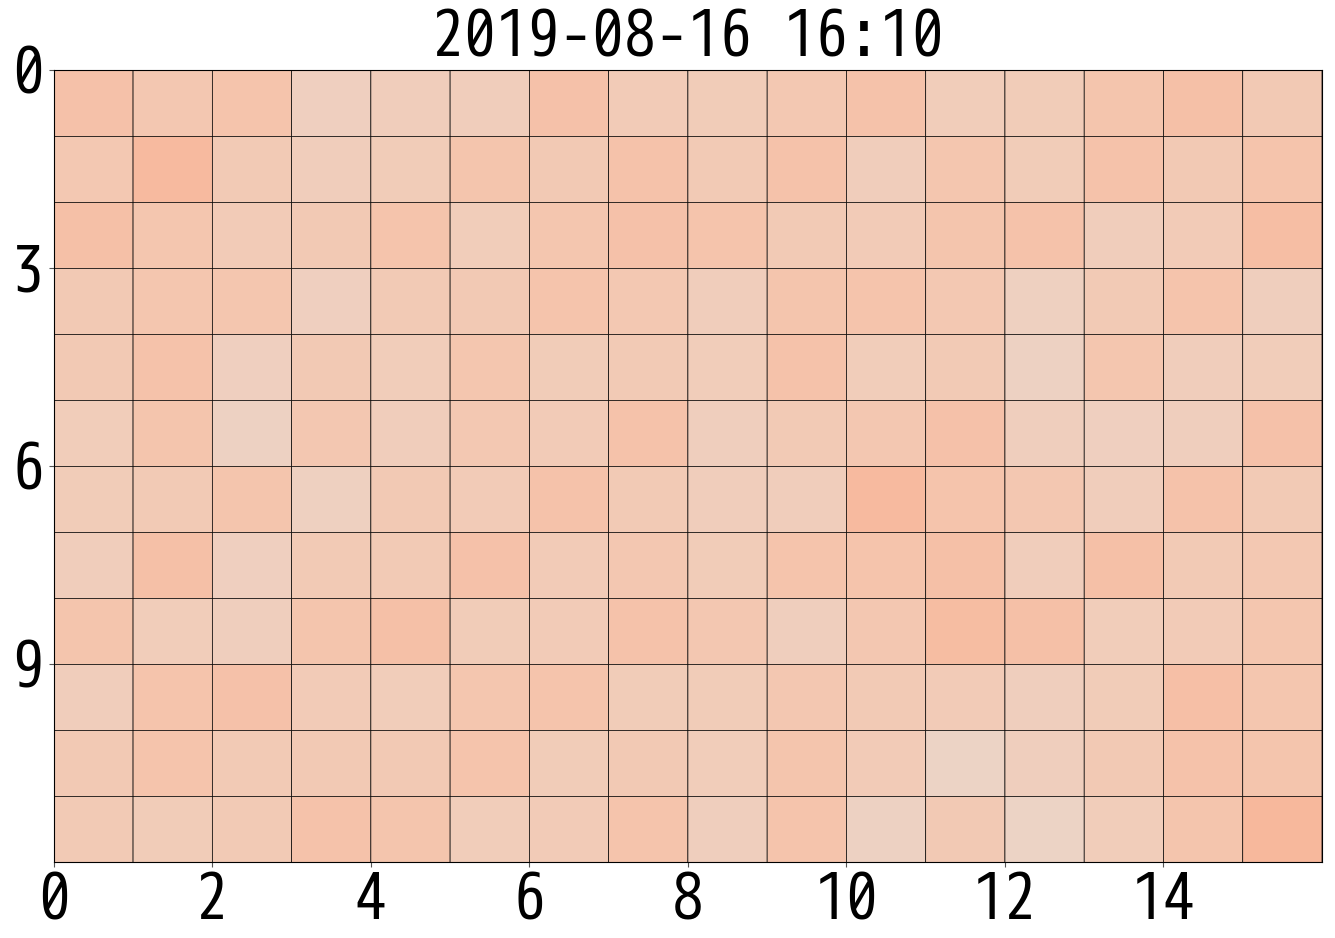
\includegraphics[width=0.98\textwidth]{IOR-OST_bw_hmap-TP-earth-agg0-rr0-req0-write-mod.png}
 \subcaption{{\tt T:agg=0,rr=0,req=0}}
 \label{fig:IOR_OST_WR_AGG0_RR0_REQ0}
\end{minipage}
%
\noindent
\begin{minipage}[t]{0.3\textwidth}
 \centering
 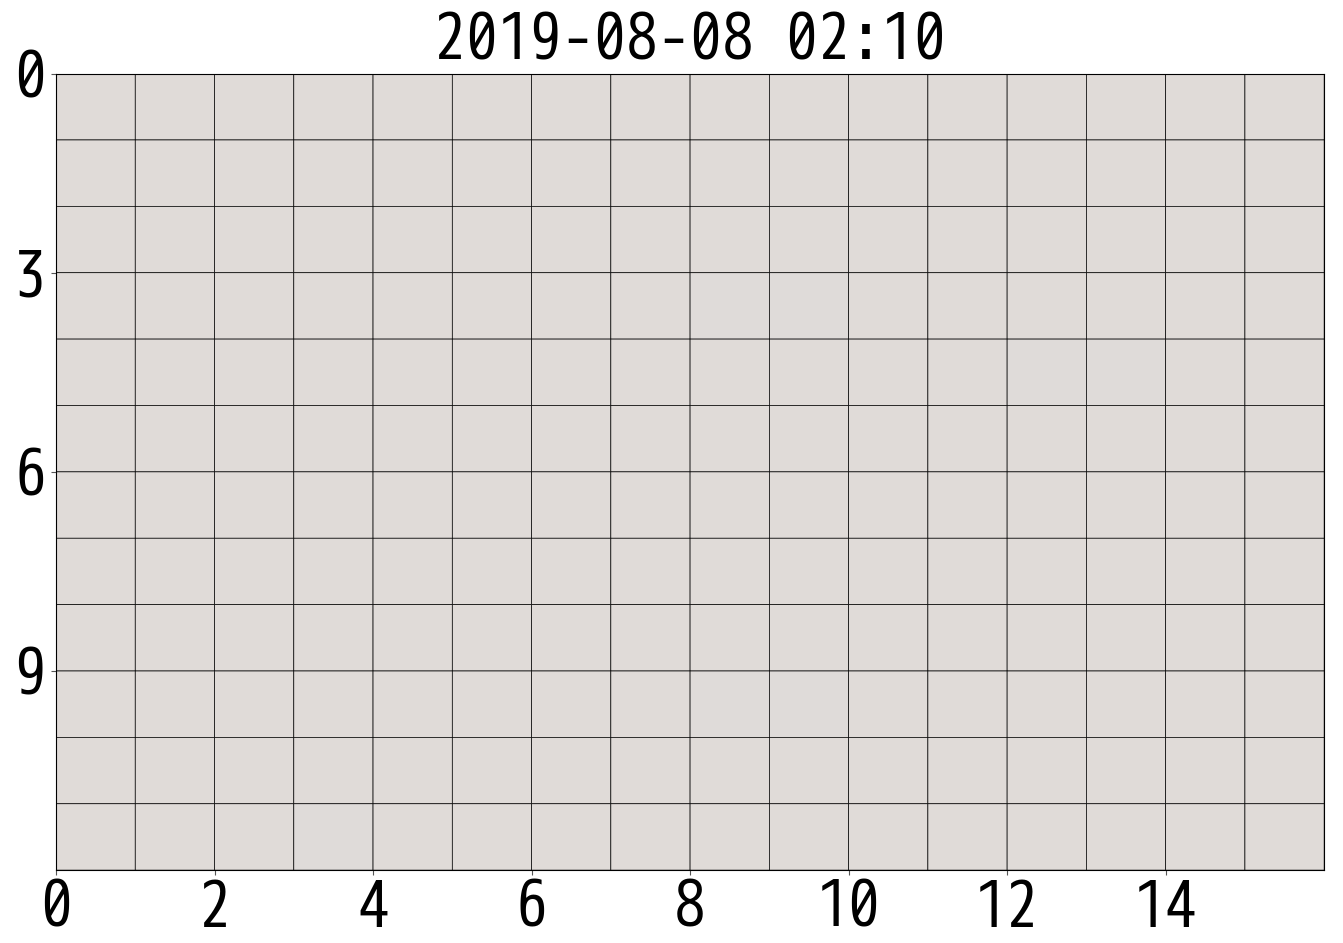
\includegraphics[width=0.98\textwidth]{IOR-OST_bw_hmap-TP-earth-agg1-rr1-req4-write-mod.png}
 \subcaption{{\tt T:agg=1,rr=1,req=4}}
 \label{fig:IOR_OST_WR_AGG1_RR1_REQ4}
\end{minipage}
%
\begin{minipage}[t]{0.3\textwidth}
 \centering
 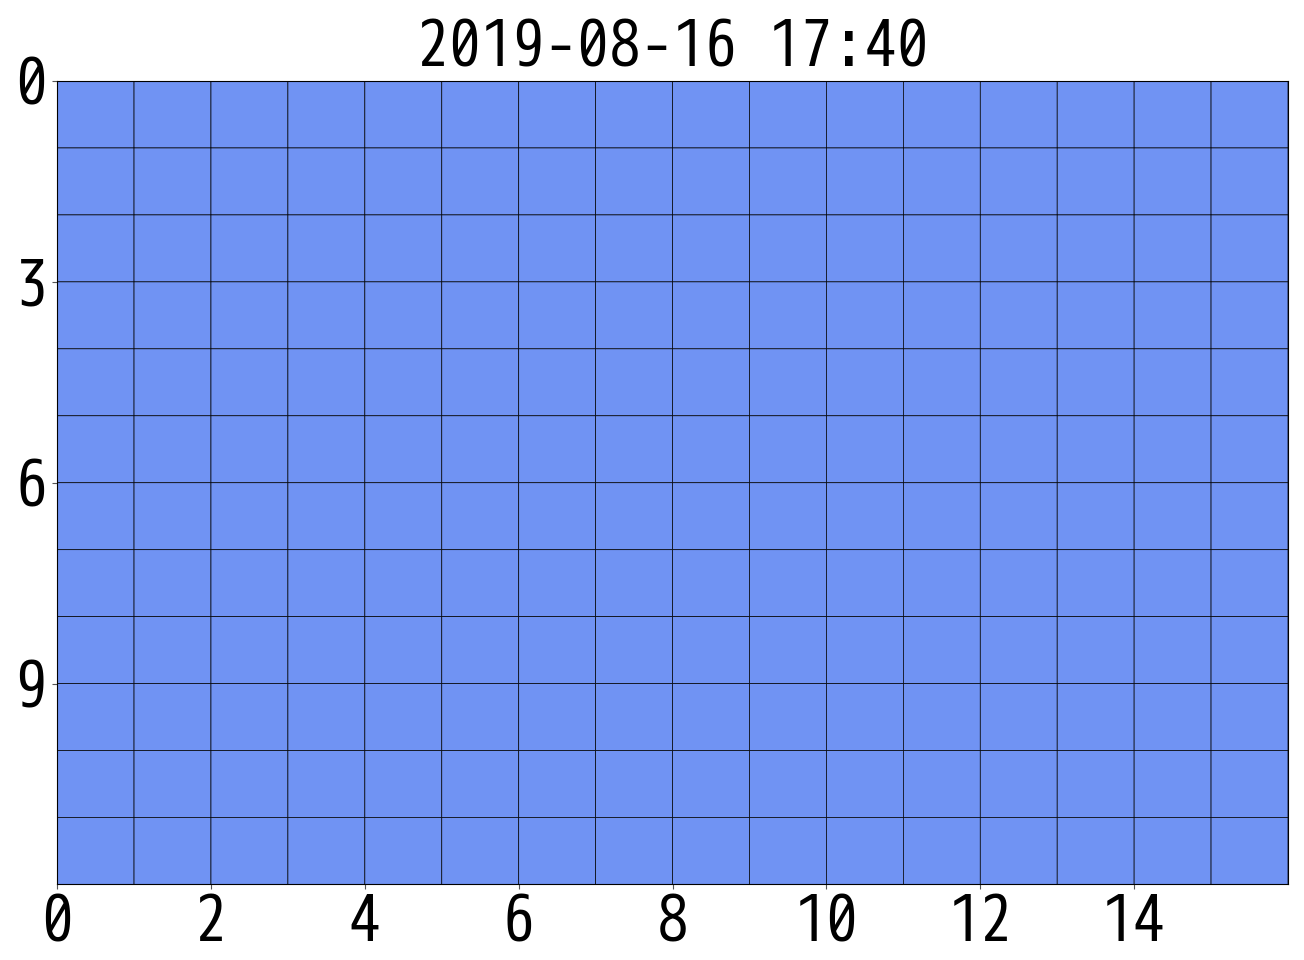
\includegraphics[width=0.98\textwidth]{IOR-OST_bw_hmap-Non_TP-orig-write-mod.png}
 \subcaption{{\tt N:original}}
 \label{fig:IOR_OST_WR_NTP_ORIG}
\end{minipage}
%
\begin{minipage}[t]{0.3\textwidth}
 \centering
 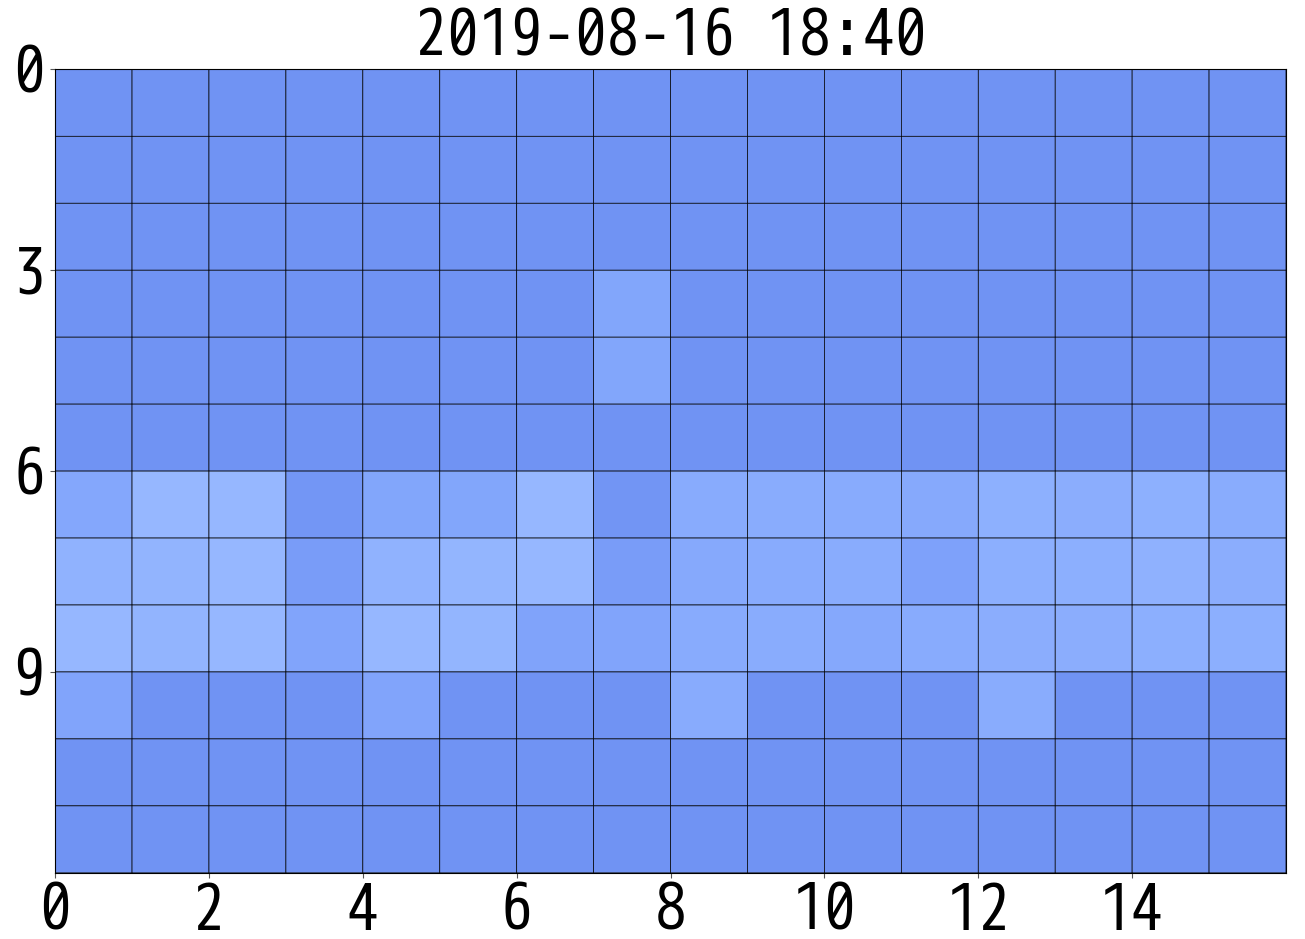
\includegraphics[width=0.98\textwidth]{IOR-OST_bw_hmap-Non_TP-earth-agg0-rr0-req4-write-mod.png}
 \subcaption{{\tt N:agg=0,rr=0,req=4}}
 \label{fig:IOR_OST_WR_NTP_AGG0_RR0_REQ4}
\end{minipage}
%
\caption{Write throughput heat-maps ranging from 0 to 160\,MiB/s
about the 192 OSTs used during the IOR benchmark run}
\label{fig:IOR_OST_BW_HMAP_WR}
\end{figure}
%
% Each heat-map showed write throughput of each OST ranging from 0 to 160\,MiB/s,
% where
Horizontal and vertical axes ranging from 0 to 15 and from 0 to 11,
indicate subjected relative 2D positions of OSTs used from the logical 3D layout
of the K computer.

In the original MPI-IO use case in Fig.~\ref{fig:IOR_OST_WR_ORIG},
we can see performance gaps among the left and right sides separated by
the dotted line.
Fig.~\ref{fig:IOR_OST_WR_AGG0_RR0_REQ0}
also shows performance gaps among OSTs used
because of imbalanced aggregator layout although the EARTH was used.
Both cases were not suitable configurations because total I/O performance
was limited by the slowest OSTs in parallel I/O.
Meanwhile, the most optimized case in Fig.~\ref{fig:IOR_OST_WR_AGG1_RR1_REQ4}
shows a well-balanced situation in write throughput among OSTs used.
Within the context of parallel I/O characteristics,
this case was suitable to achieve I/O performance for the benchmark run.

On the other hand,
Figs.~\ref{fig:IOR_OST_WR_NTP_ORIG} and
\ref{fig:IOR_OST_WR_NTP_AGG0_RR0_REQ4} show poor I/O throughput
in collective write operations in the original and the EARTH use cases
without two-phase I/O, respectively.
These poor performance situations were due to contention
in I/O task assignment to I/O threads by huge number of concurrent I/O accesses
from all 12,288 processes as we observed in
Figs.~\ref{fig:IOR_req_qdepth} and \ref{fig:IOR_req_waittime}.

Figure~\ref{fig:IOR_OST_BW_HMAP_RD} shows read throughput heat-maps
ranging from 0 to 160\,MiB/s among the 192 OSTs used at the IOR benchmark runs.
%
\begin{figure}[tb]
\begin{minipage}[t]{0.06\textwidth}
 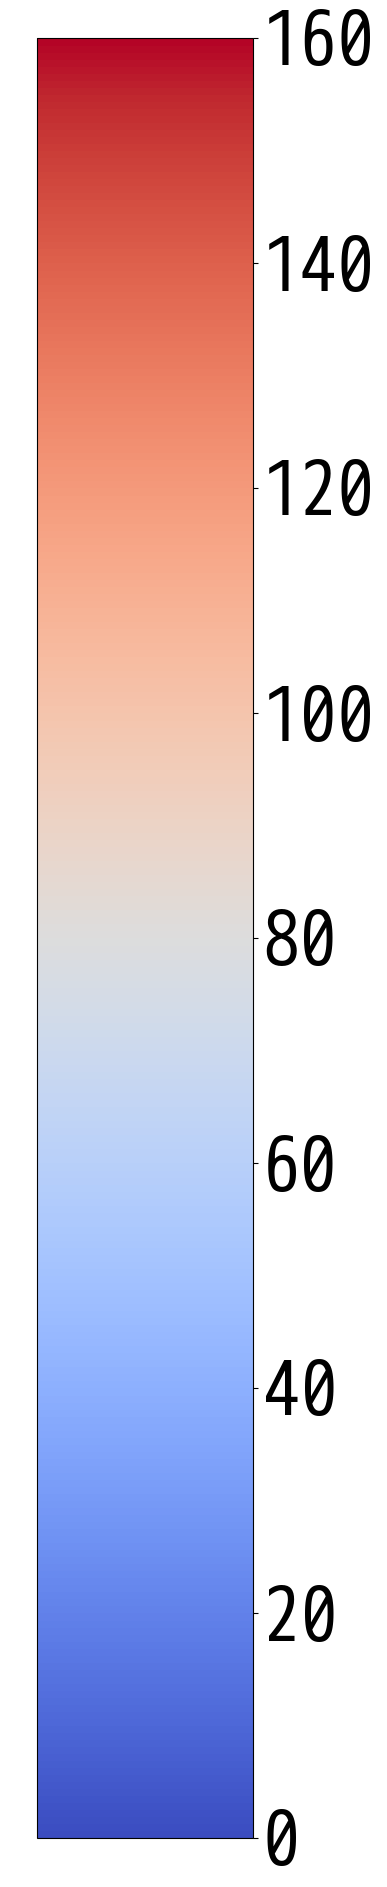
\includegraphics[width=0.98\textwidth,height=0.14\textheight]{hmap-colorbar-mod2.png}
\end{minipage}
%
\noindent
\begin{minipage}[t]{0.3\textwidth}
 \centering
 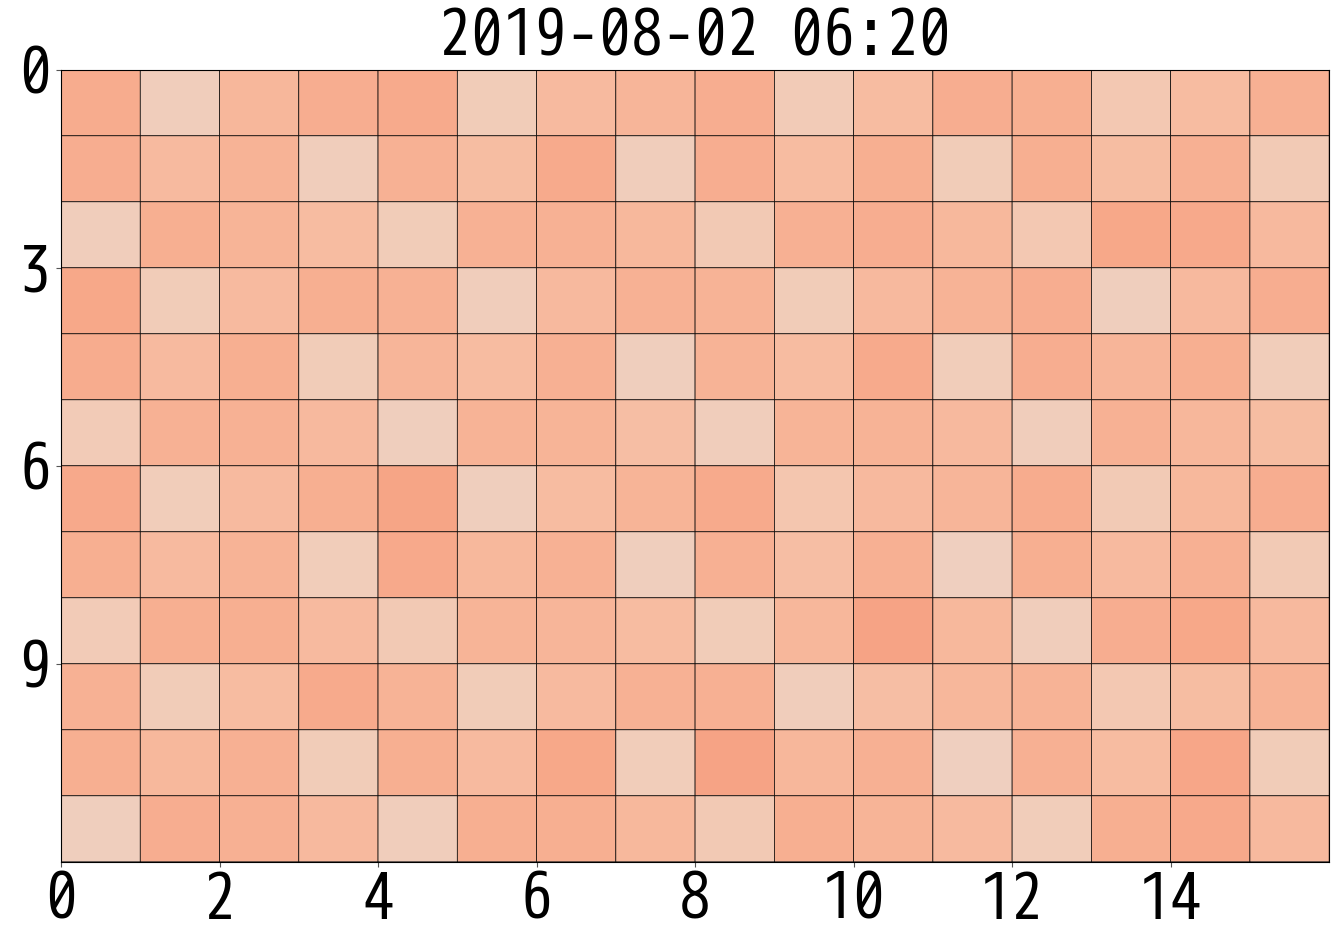
\includegraphics[width=0.98\textwidth]{IOR-OST_bw_hmap-TP-orig-read-mod.png}
 \subcaption{{\tt T:original}}
 \label{fig:IOR_OST_RD_ORIG}
\end{minipage}
%
\noindent
\begin{minipage}[t]{0.3\textwidth}
 \centering
 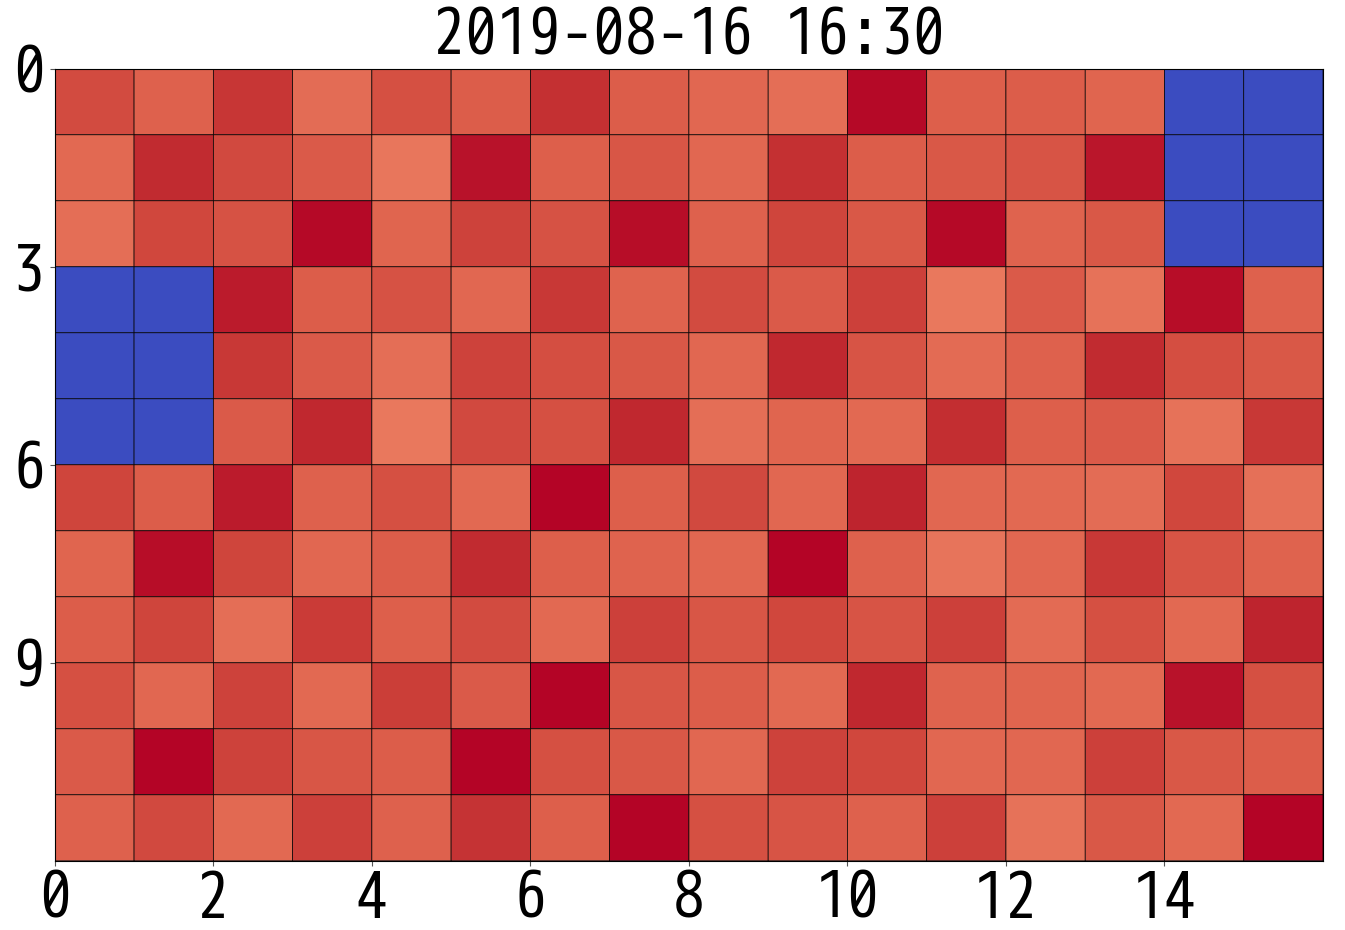
\includegraphics[width=0.98\textwidth]{IOR-OST_bw_hmap-TP-earth-agg0-rr0-req0-read-mod.png}
 \subcaption{{\tt T:agg=0,rr=0,req=0}}
 \label{fig:IOR_OST_RD_AGG0_RR0_REQ0}
\end{minipage}
%
\noindent
\begin{minipage}[t]{0.3\textwidth}
 \centering
 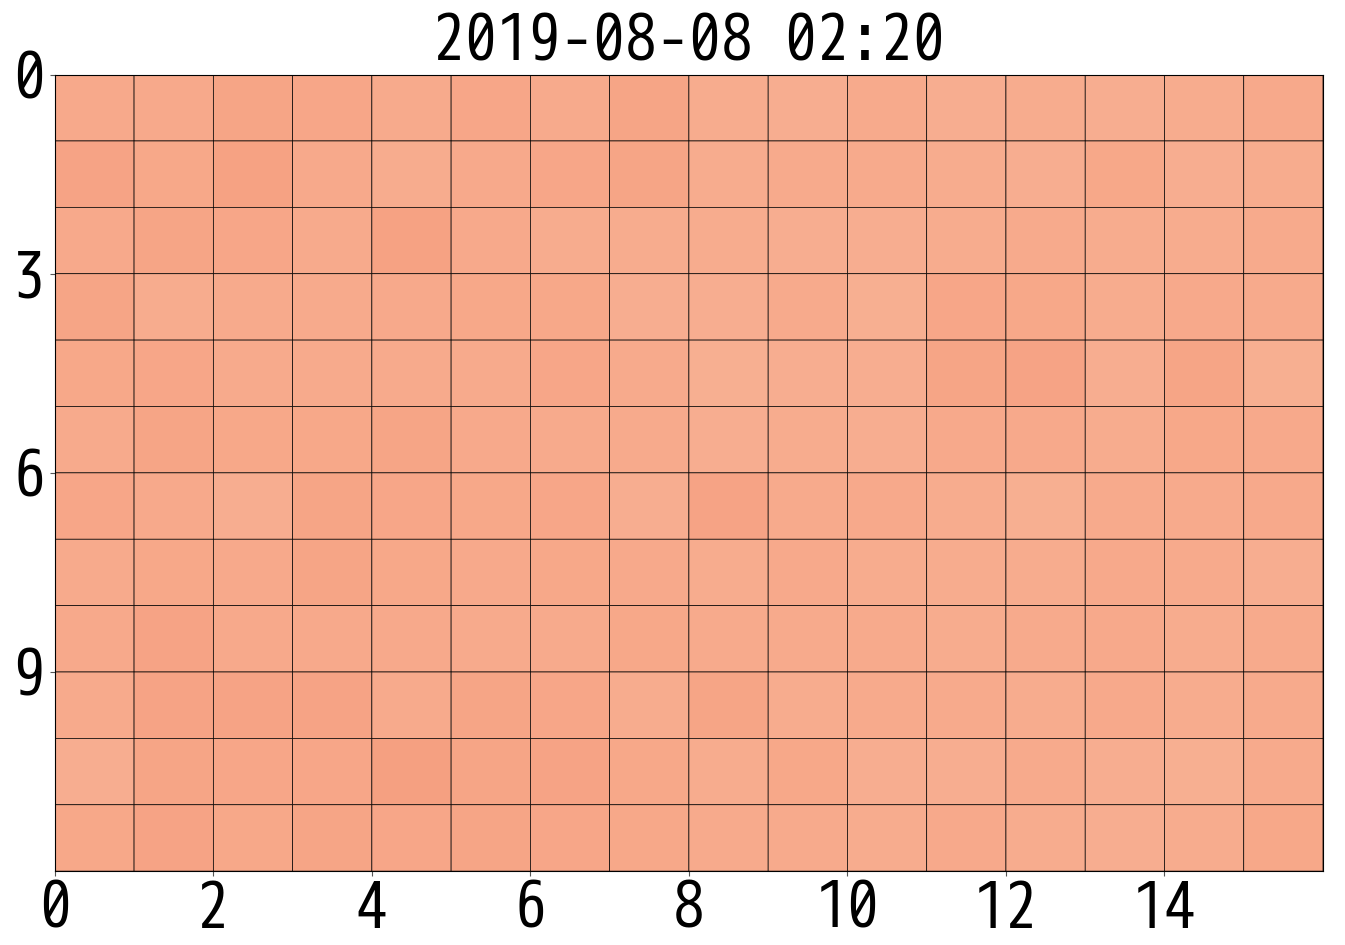
\includegraphics[width=0.98\textwidth]{IOR-OST_bw_hmap-TP-earth-agg1-rr1-req4-read-mod.png}
 \subcaption{{\tt T:agg=1,rr=1,req=4}}
 \label{fig:IOR_OST_RD_AGG1_RR1_REQ4}
\end{minipage}
%
\begin{minipage}[t]{0.3\textwidth}
 \centering
 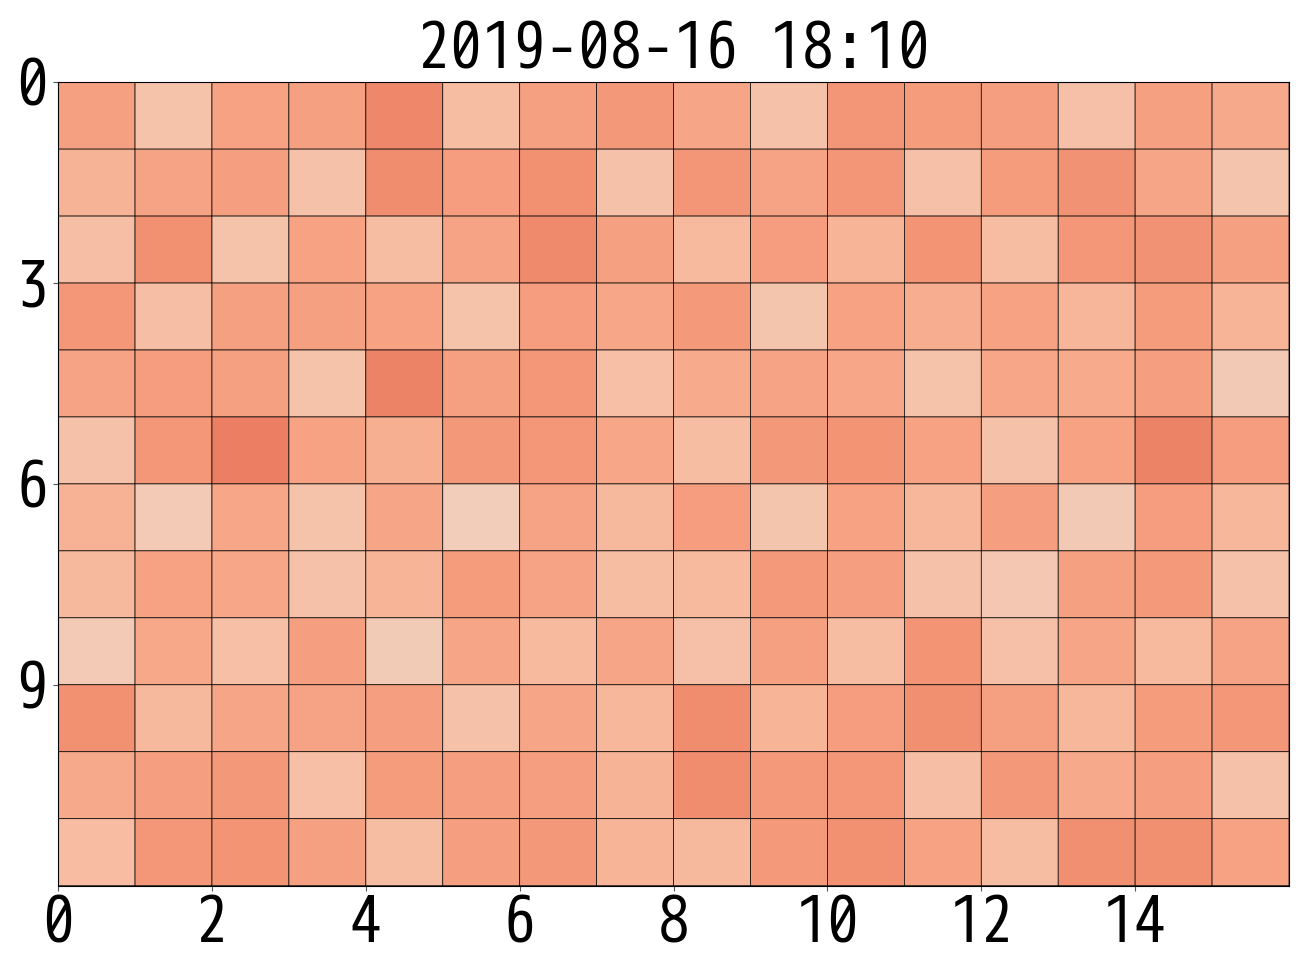
\includegraphics[width=0.98\textwidth]{IOR-OST_bw_hmap-Non_TP-orig-read-mod.png}
 \subcaption{{\tt N:original}}
 \label{fig:IOR_OST_RD_NTP_ORIG}
\end{minipage}
%
\begin{minipage}[t]{0.3\textwidth}
 \centering
 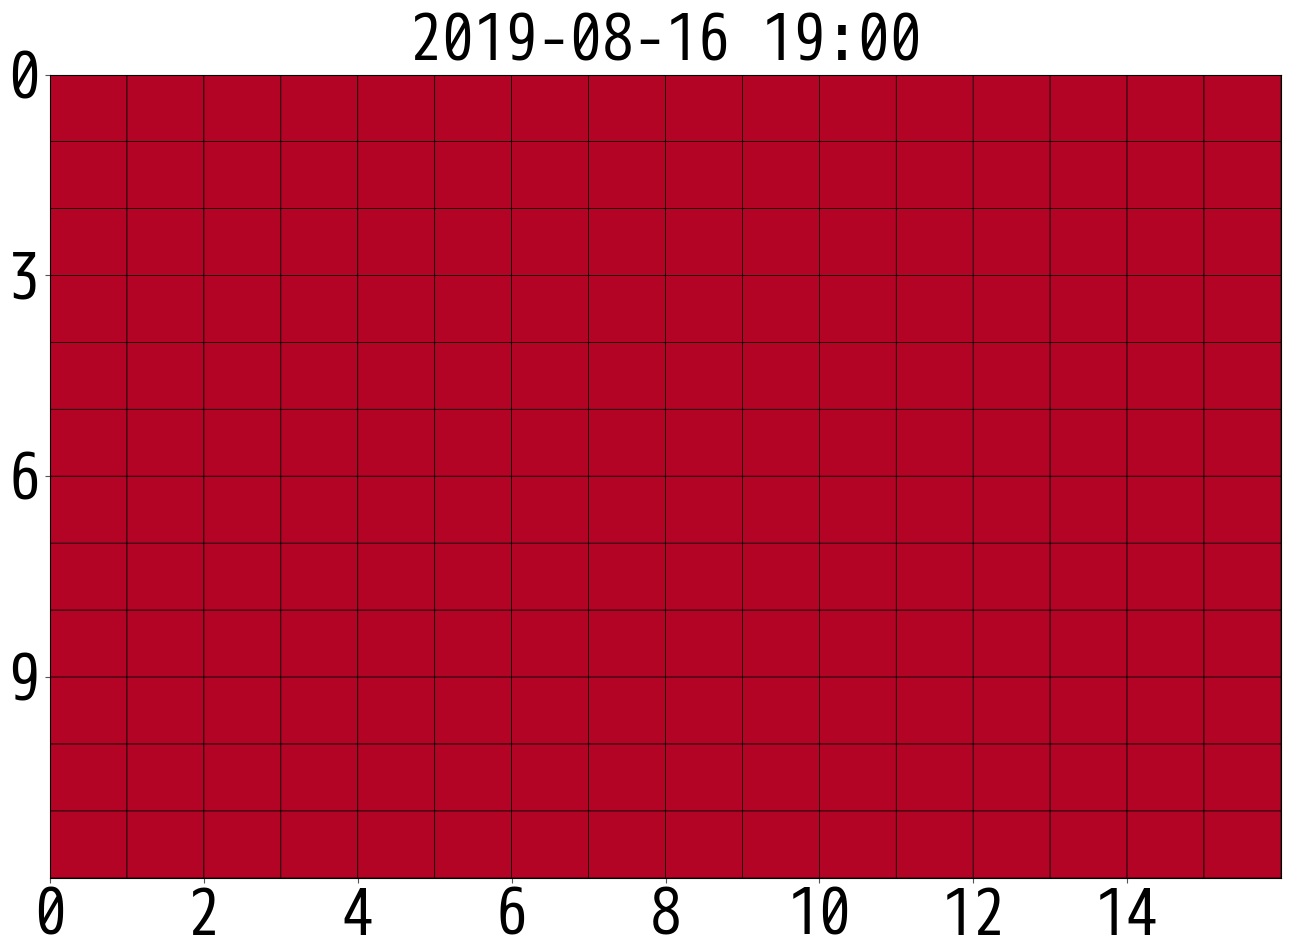
\includegraphics[width=0.98\textwidth]{IOR-OST_bw_hmap-Non_TP-earth-agg0-rr0-req4-read-mod.png}
 \subcaption{{\tt N:agg=0,rr=0,req=4}}
 \label{fig:IOR_OST_RD_NTP_AGG0_RR0_REQ4}
\end{minipage}
%
\caption{Read throughput heat-maps ranging from 0 to 160\,MiB/s
about the 192 OSTs used during the IOR benchmark run}
\label{fig:IOR_OST_BW_HMAP_RD}
\end{figure}
%
Imbalanced bandwidth situations in the original MPI-IO use case
and the EARTH use case without any optimizations were observed
in Figs.~\ref{fig:IOR_OST_RD_ORIG} and \ref{fig:IOR_OST_RD_AGG0_RR0_REQ0}, respectively.
Meanwhile, well-balanced situations were achieved in the EARTH use case
with an optimal optimization configuration,
which led to high performance collective I/O,
as shown in Fig.~\ref{fig:IOR_OST_RD_AGG1_RR1_REQ4}.

Write and read throughput heat-maps ranging from 0 to 160\,MiB/s
at the HPIO run are also shown in
Figs.~\ref{fig:HPIO_OST_BW_HMAP_WR} and \ref{fig:HPIO_OST_BW_HMAP_RD}, respectively.
%
\begin{figure}[tb]
\begin{minipage}[t]{0.06\textwidth}
 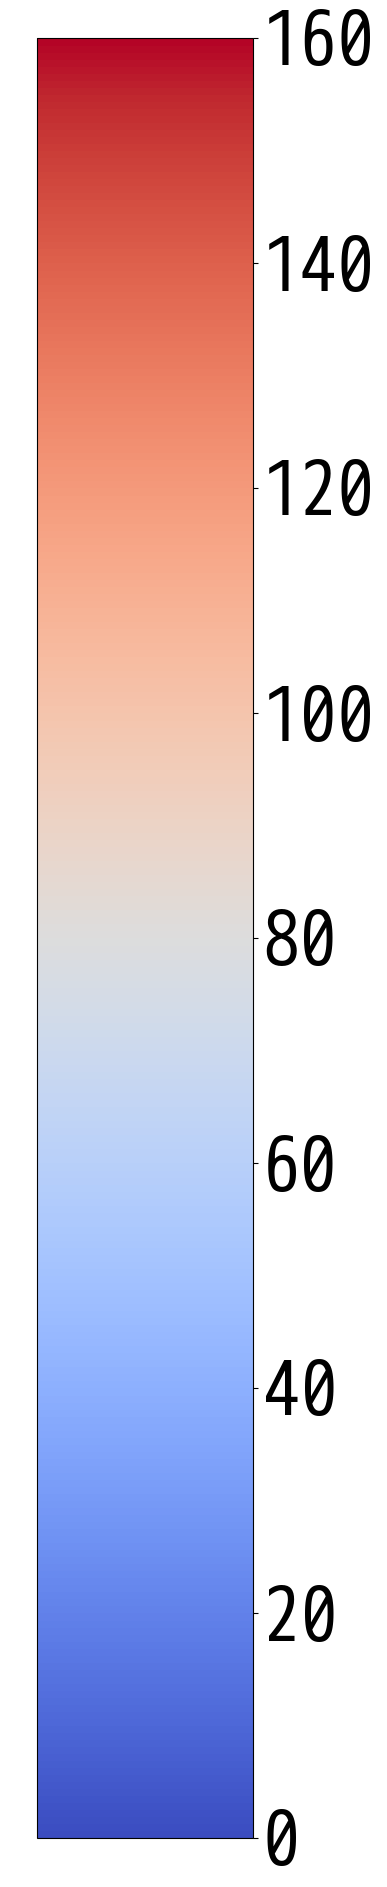
\includegraphics[width=0.98\textwidth,height=0.14\textheight]{hmap-colorbar-mod2.png}
\end{minipage}
%
\noindent
\begin{minipage}[t]{0.29\textwidth}
 \centering
 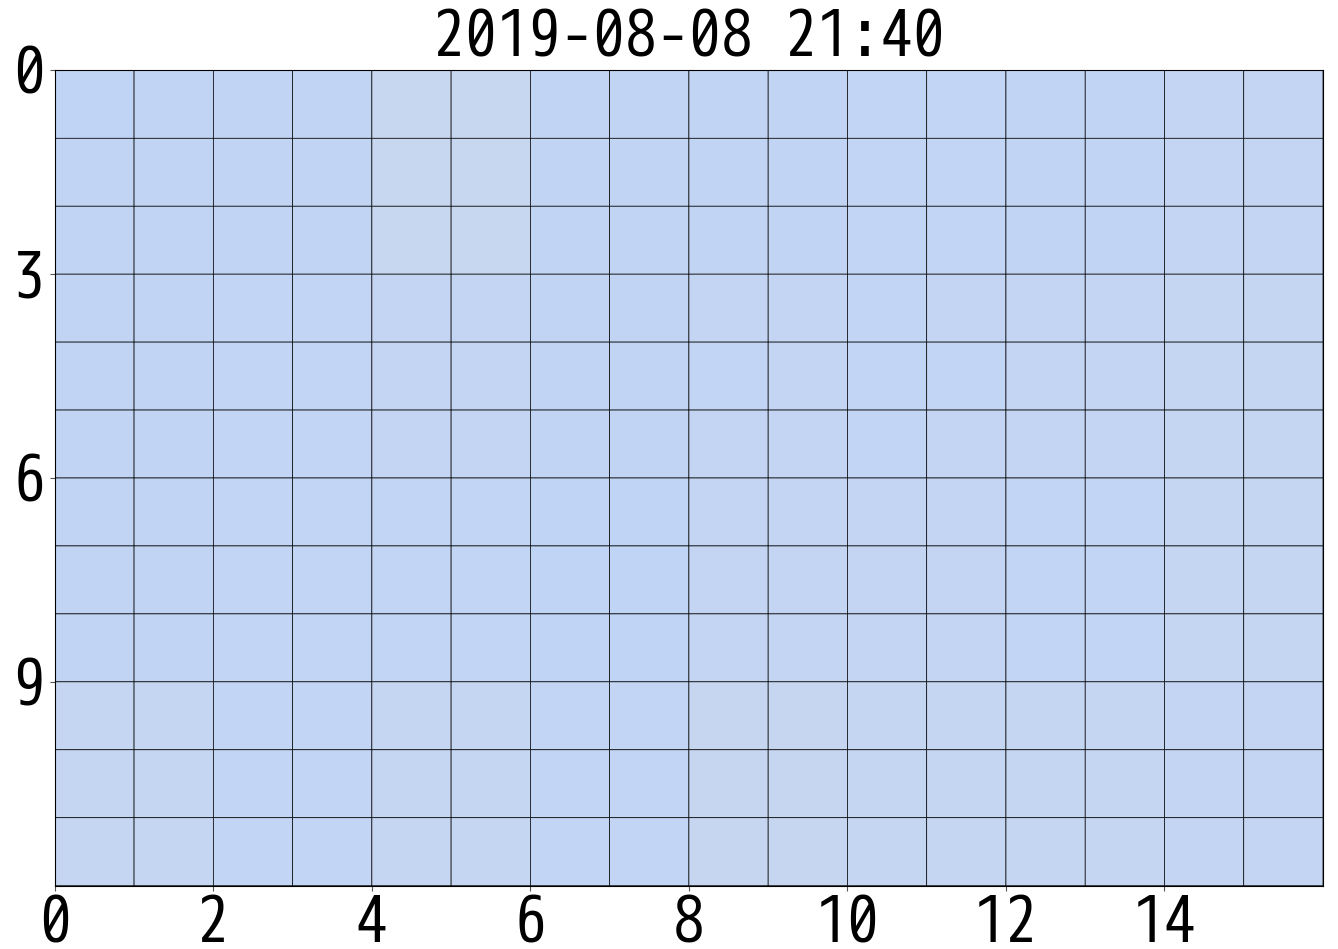
\includegraphics[width=0.96\textwidth]{hpio-OST_bw_hmap-orig-write-mod.png}
 \subcaption{{\tt T:original}}
\end{minipage}
%
\noindent
\begin{minipage}[t]{0.29\textwidth}
 \centering
 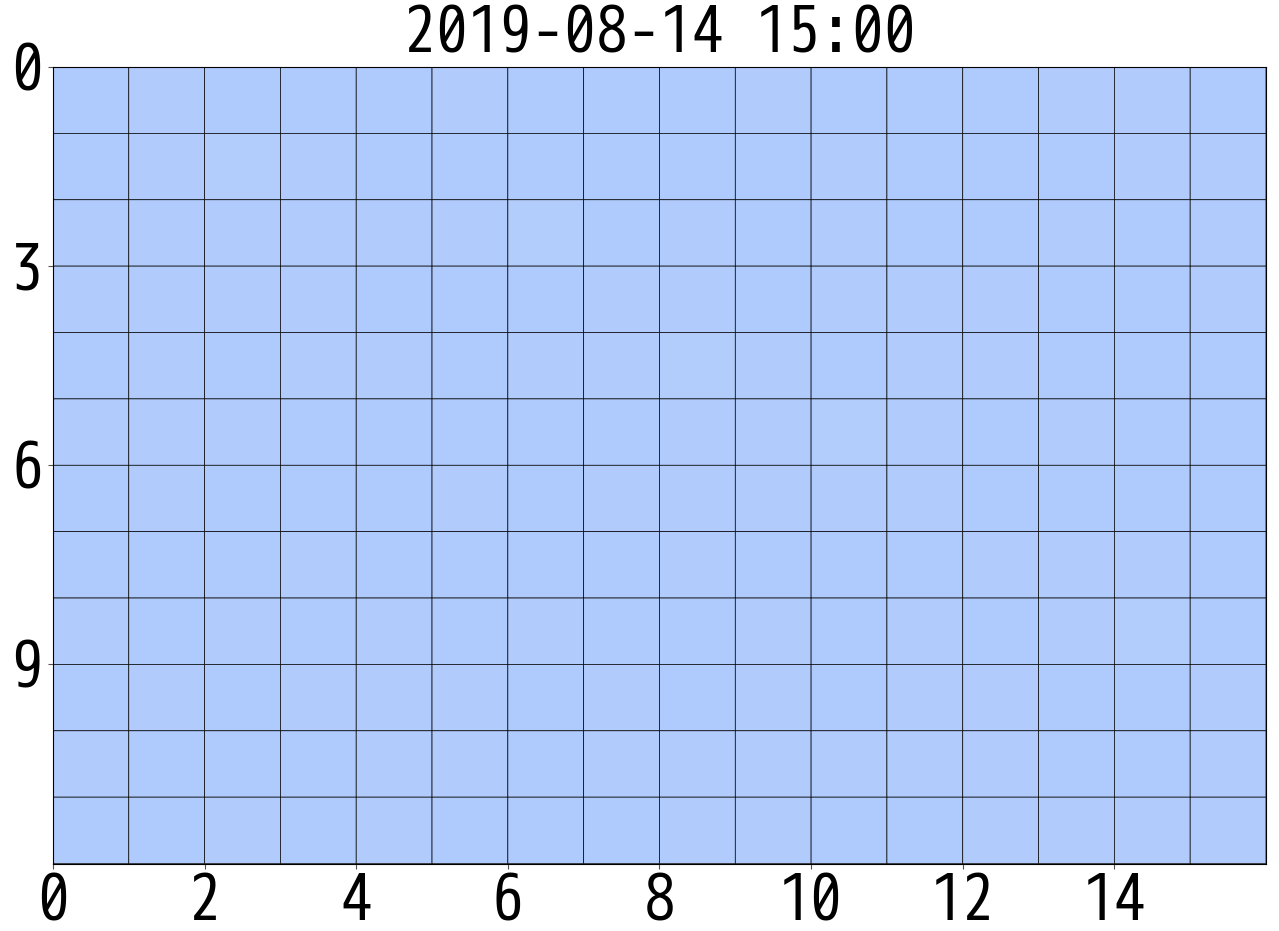
\includegraphics[width=0.96\textwidth]{hpio-OST_bw_hmap-earth-agg0-rr0-req8-write-mod.png}
 \subcaption{{\tt T:agg=0,rr=0,req=8}}
\end{minipage}
%
\noindent
\begin{minipage}[t]{0.31\textwidth}
 \centering
 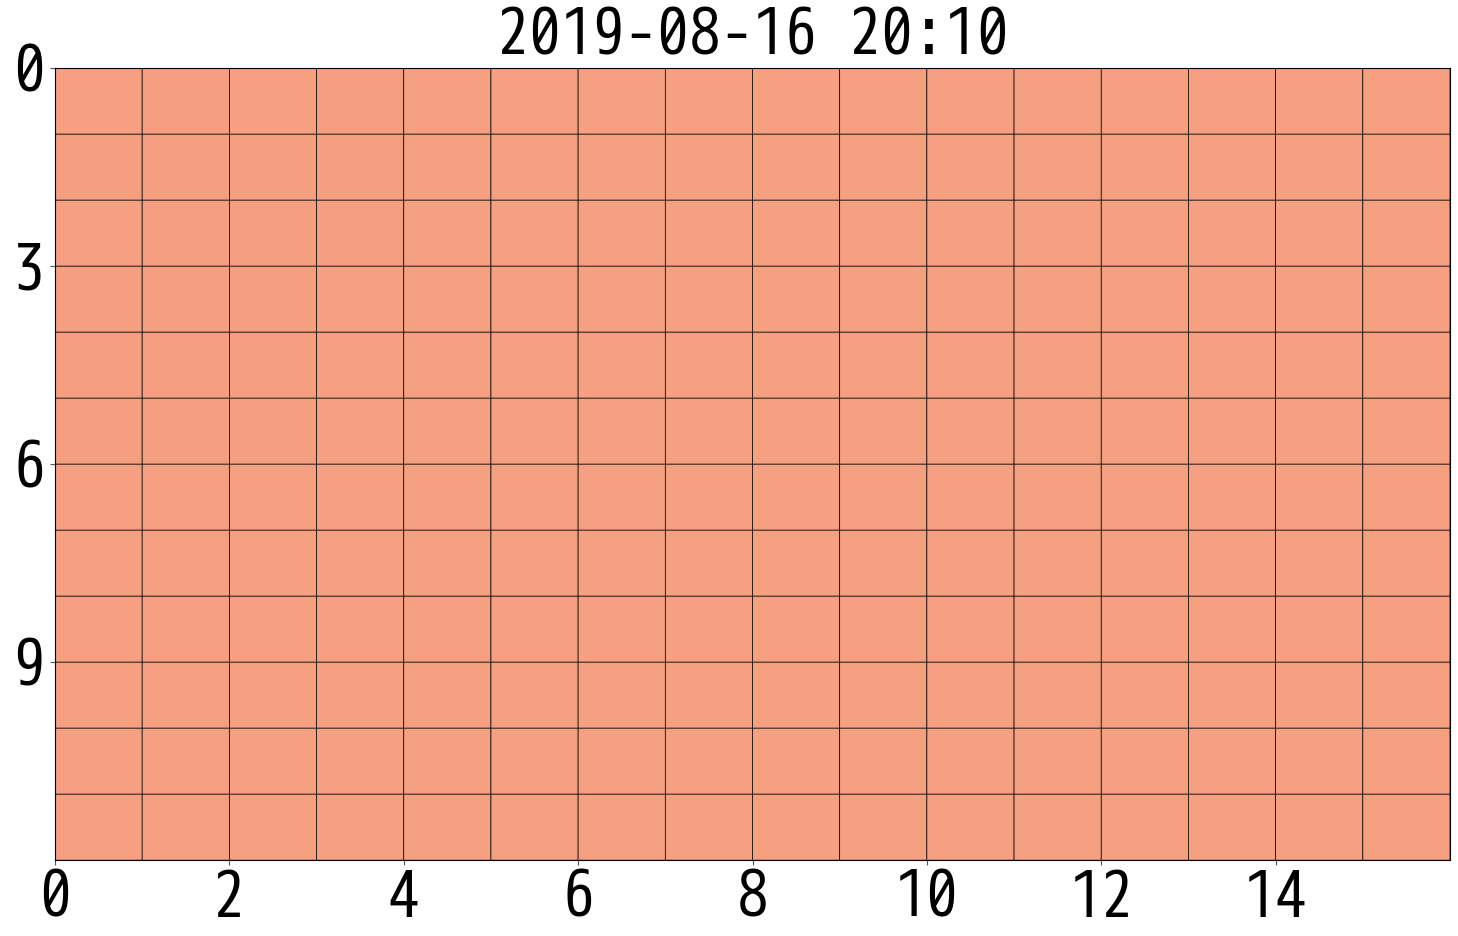
\includegraphics[width=1.0\textwidth]{hpio-OST_bw_hmap-earth-agg1-rr1-req8-write-mod.png}
 \subcaption{{\tt T:agg=1,rr=1,req=8}}
\end{minipage}
%
\caption{Write throughput heat-maps ranging from 0 to 160\,MiB/s about
the 192 OSTs used at the HPIO benchmark run}
\label{fig:HPIO_OST_BW_HMAP_WR}
\end{figure}
%
\begin{figure}[tb]
\begin{minipage}[t]{0.06\textwidth}
 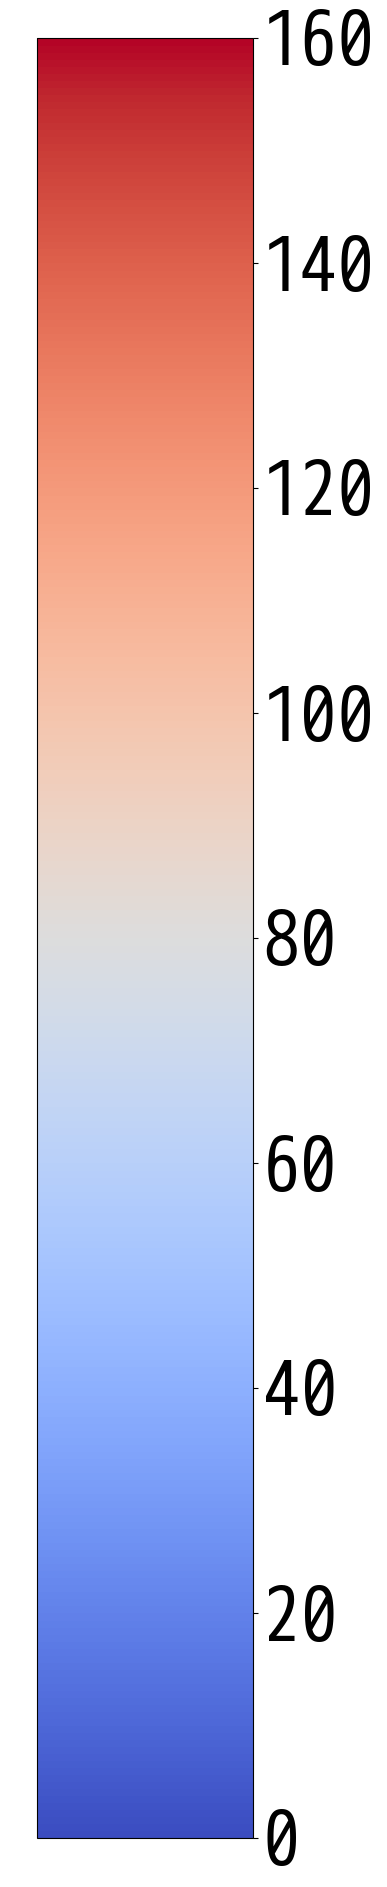
\includegraphics[width=0.98\textwidth,height=0.14\textheight]{hmap-colorbar-mod2.png}
\end{minipage}
%
\noindent
\begin{minipage}[t]{0.29\textwidth}
 \centering
 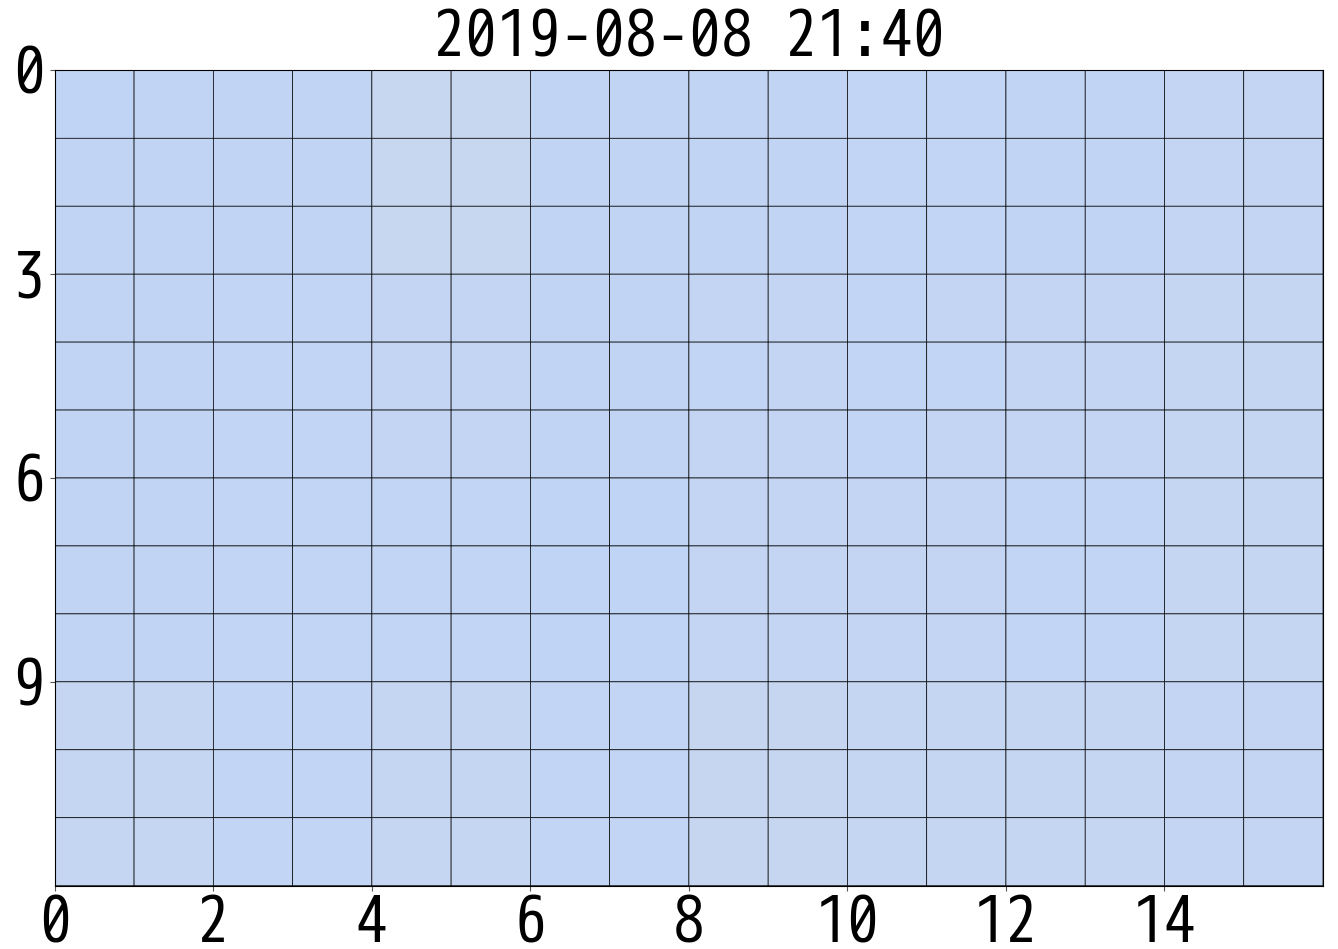
\includegraphics[width=0.96\textwidth]{hpio-OST_bw_hmap-orig-write-mod.png}
 \subcaption{{\tt T:original}}
\end{minipage}
%
\noindent
\begin{minipage}[t]{0.29\textwidth}
 \centering
 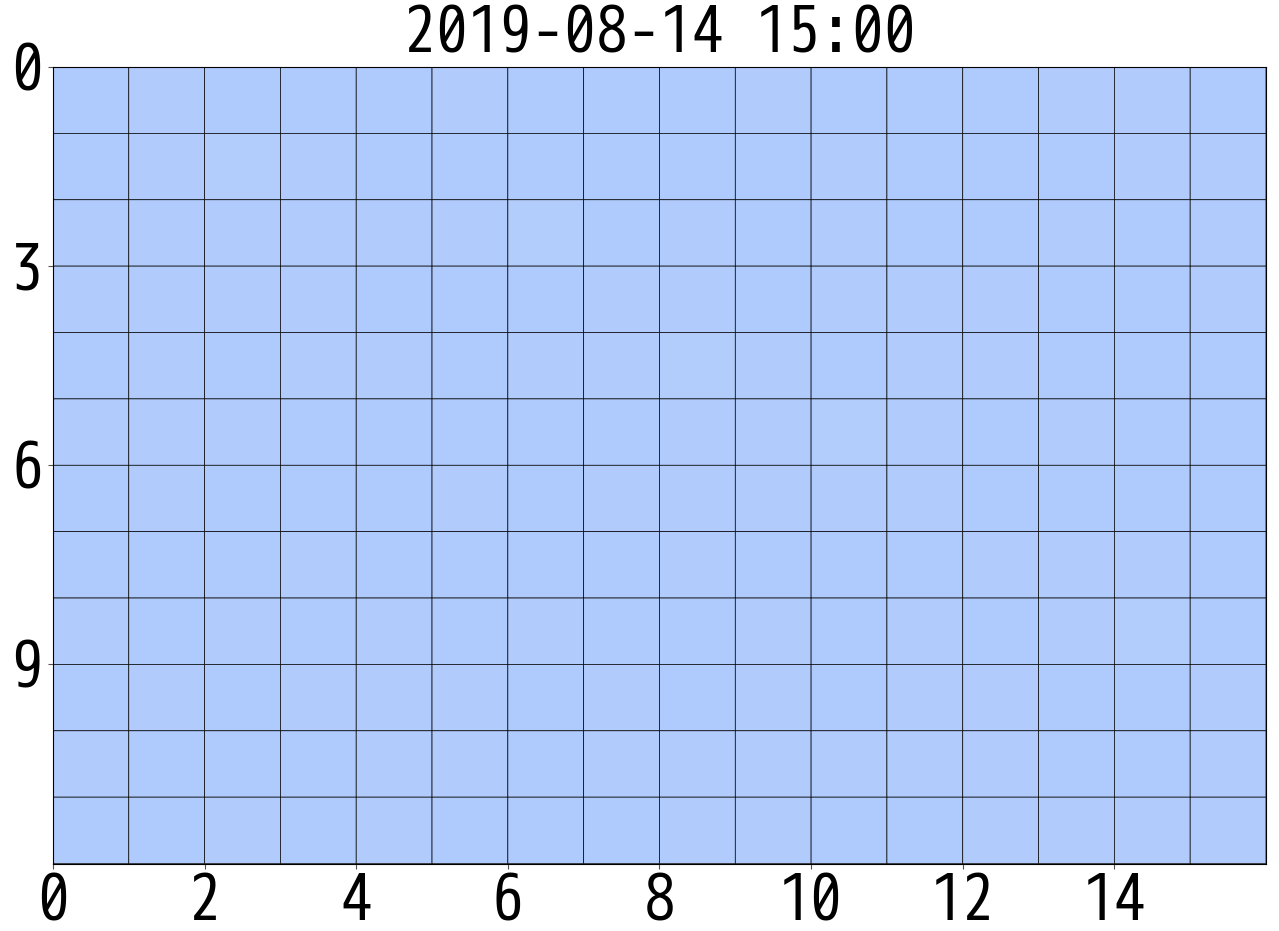
\includegraphics[width=0.96\textwidth]{hpio-OST_bw_hmap-earth-agg0-rr0-req8-write-mod.png}
 \subcaption{{\tt T:agg=0,rr=0,req=8}}
\end{minipage}
%
\noindent
\begin{minipage}[t]{0.31\textwidth}
 \centering
 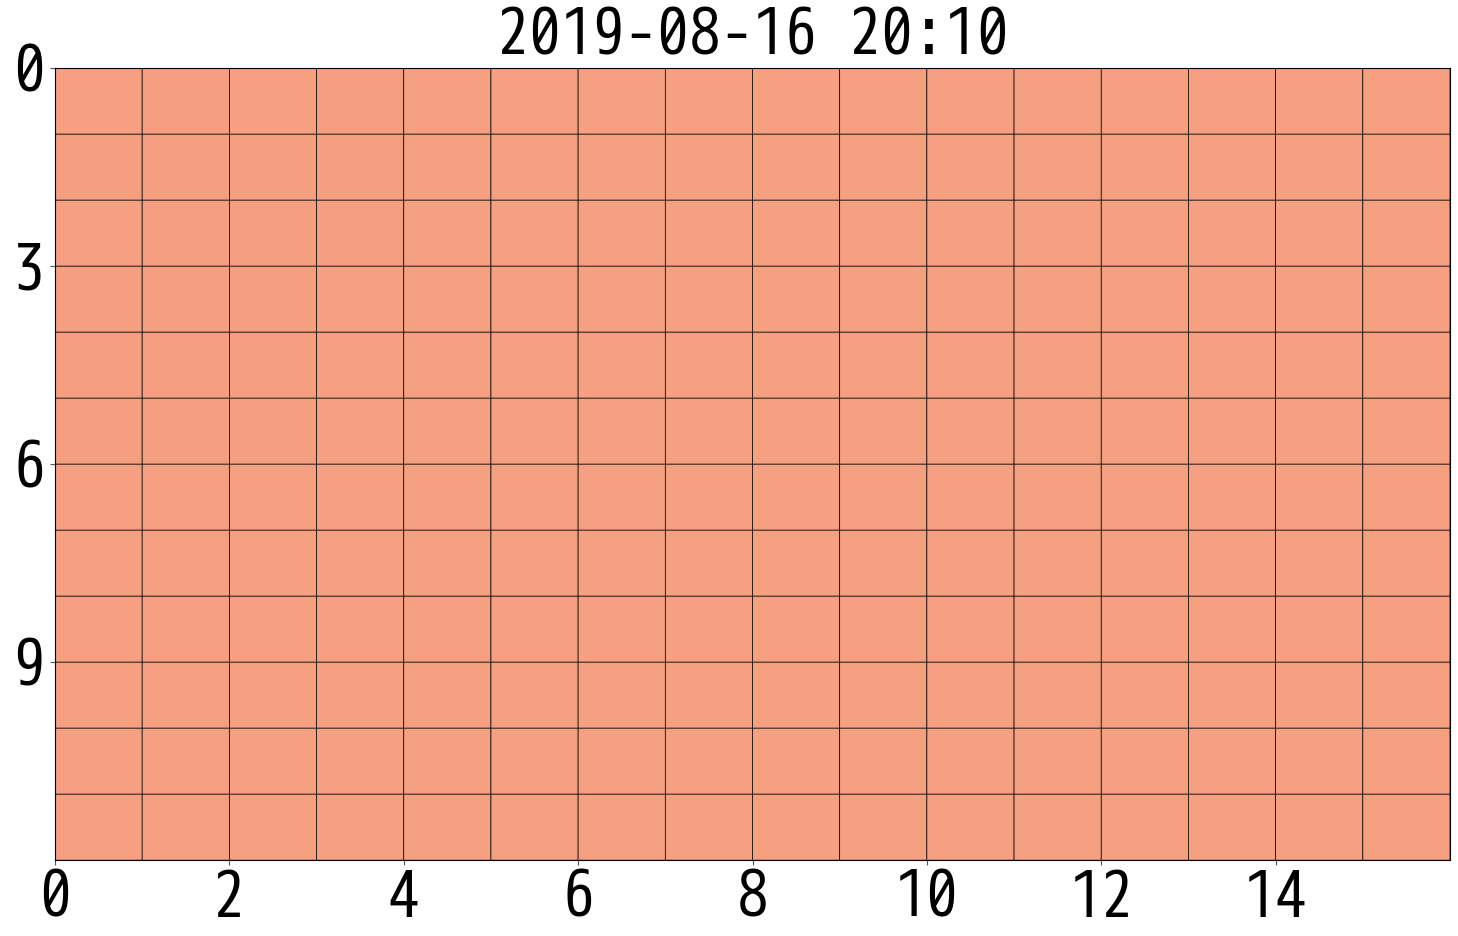
\includegraphics[width=1.0\textwidth]{hpio-OST_bw_hmap-earth-agg1-rr1-req8-write-mod.png}
 \subcaption{{\tt T:agg=1,rr=1,req=8}}
\end{minipage}
%
\caption{Read throughput heat-maps ranging from 0 to 160\,MiB/s about
the 192 OSTs used at the HPIO benchmark run}
\label{fig:HPIO_OST_BW_HMAP_RD}
\end{figure}
%
In Fig.~\ref{fig:HPIO_OST_BW_HMAP_RD}, the EARTH use case with insufficient configuration
({\tt T:agg=0,rr=0,req=8}) showed lower performance compared with the original MPI-IO use case.
Meanwhile, a full set of the three optimizations in the EARTH use case
({\tt T:agg=1,rr=1,req=8}) achieved the highest I/O throughput at every used OST. 
Read throughput heat-maps in Fig.~\ref{fig:HPIO_OST_BW_HMAP_RD} show
the highest I/O throughput in the insufficient optimization configuration
({\tt T:agg=0,rr=0,req=8}), followed by the original MPI-IO use case
and the full optimization configuration case.
However, the insufficient configuration case performed the longest waiting time
in the Tofu interconnects among the I/O nodes used,
as shown in Fig.~\ref{fig:HPIO_ION_TOFU_WAIT_TIME},
and thus high I/O bandwidth could not be achieved in this configuration.

\subsection{Overall evaluation}
\label{ssec:overall_eval}

We conducted the overall evaluation based on the abovementioned results
in each target metric.
From the results in write and read operations in each benchmark run,
we obtained mean values of the following metrics:
%
\begin{itemize}
\item Three metrics of {\tt I/O stats}:
({\tt req\_qdepth}, {\tt req\_waittime}, and {\tt req\_active})
\item Two metrics of {\tt Tofu stats}: ($R_{BW}$ and $T_{wait}^{max}$)
\item Mean OST I/O bandwidth from {\tt I/O rates} ($OST_{mean}$)
\end{itemize}
%
It is preferable to have low values in the two of the three metrics
in {\tt I/O stats}, {\tt req\_qdepth} and {\tt req\_waittime}.
While having high value is preferable in the {\tt req\_active}.
Concerning the two metrics in the {\tt Tofu stats},
high value is desirable in $R_{BW}$, while low value is
suitable in $T_{wait}^{max}$.
High value is preferable in $OST_{mean}$ from {\tt I/O rates}.
We gave them ranks from 1 in the order from the best one
among the evaluated optimizations in each metric according to
the above context.
Finally we obtained a stats score as a mean value of the ranks.

Table~\ref{tbl:IOR_OVERALL_EVAL} summarizes the scores of the IOR benchmark run.
%
\begin{table}[tb]
\caption{Scores of the IOR benchmark run, where lesser is better in each score number}
\centering
\begin{tabular}{lccccccc}
\hline
\multicolumn{1}{c}{Optimization}  & \multicolumn{3}{c}{{\tt I/O stats}} & \multicolumn{2}{c}{{\tt Tofu stats}} & {\tt I/O rates} & Overall \\
\multicolumn{1}{c}{configuration} & {\tt req\_qdepth} & {\tt req\_waittime} & {\tt req\_active} &  $R_{BW}$ & $T_{wait}^{max}$ & $OST_{mean}$ & score \\
\hline
T:original          & 7 & 7 & 1 & 7 & 2 & 5 & 4.83 \\
T:agg=0,rr=0,req=0  & 5 & 4 & 4 & 6 & 7 & 1 & 4.50 \\
T:agg=0,rr=0,req=4  & 1 & 1 & 8 & 4 & 8 & 7 & 4.83 \\
T:agg=1,rr=0,req=4  & 2 & 2 & 5 & 2 & 5 & 6 & 3.67 \\
T:agg=1,rr=1,req=4  & 3 & 3 & 3 & 1 & 6 & 4 & 3.33 \\
T:agg=1,rr=1,req=16 & 6 & 5 & 2 & 3 & 4 & 2 & 3.67 \\
N:original          & 8 & 8 & 6 & 8 & 1 & 8 & 6.50 \\
N:agg=0,rr=0,req=4  & 4 & 6 & 7 & 5 & 3 & 3 & 4.67 \\
\hline
\end{tabular}
\label{tbl:IOR_OVERALL_EVAL}
\end{table}
%
We can see that the case of {\tt T:agg=1,rr=1,req=4} shows
the best overall score (3.33) among the evaluated optimization parameter sets.
Although we already examined that this case was the best in the IOR run,
we observed another insight that the bast case achieved such balanced situation
among I/O subsystems from the score.
%% The best score was achieved because of the balanced scores
%% in the evaluated six metrics.

Meanwhile, the scores of the HPIO benchmark run are summarized in
Table~\ref{tbl:HPIO_OVERALL_EVAL}.
%
\begin{table}[tb]
\caption{Scores of the HPIO benchmark run, where lesser is better in each score number}
\centering
\begin{tabular}{lccccccc}
\hline
\multicolumn{1}{c}{Optimization}  & \multicolumn{3}{c}{{\tt I/O stats}} & \multicolumn{2}{c}{{\tt Tofu stats}} & {\tt I/O rates} & Overall \\
\multicolumn{1}{c}{configuration} & {\tt req\_qdepth} & {\tt req\_waittime} & {\tt req\_active} &  $R_{BW}$ & $T_{wait}^{max}$ & $OST_{mean}$ & score \\
\hline
T:original         & 5 & 6 & 2 & 5 & 1 & 5 & 4.00 \\
T:agg=0,rr=0,req=0 & 4 & 5 & 4 & 4 & 2 & 6 & 4.17 \\
T:agg=0,rr=0,req=8 & 1 & 1 & 6 & 2 & 6 & 1 & 2.83 \\
T:agg=1,rr=1,req=8 & 3 & 4 & 1 & 1 & 4 & 3 & 2.67 \\
T:agg=1,rr=1,req=2 & 2 & 2 & 5 & 3 & 3 & 4 & 3.17 \\
T:agg=1,rr=1,req=4 & 6 & 3 & 3 & 6 & 5 & 2 & 4.17 \\
\hline
\end{tabular}
\label{tbl:HPIO_OVERALL_EVAL}
\end{table}
%
From this table, we can see that the case of {\tt T:agg=1,rr=1,req=8}
achieves the best score (2.67) among the evaluated optimization parameter configurations.
The best case showed balanced situation among the I/O subsystems
as well as the IOR benchmark run.
We can easily observe the best optimization configuration with
the balanced situation using the scoring scheme.

\section{Conclusions}
\label{sec:CONCLUSIONS}

We built a holistic log data analysis framework to characterize I/O activities
at the LFS and data transfers through the Tofu interconnects of I/O nodes
in I/O optimization at the K computer.
The proposed framework utilized the bandwidth status of the Tofu links
among I/O nodes used and performance metrics of log data generated at the LFS
and I/O nodes.
The holistic analysis of data transfer activities on the Tofu links among I/O nodes
and I/O activities on the LFS provided useful information in I/O performance tuning.

The two I/O benchmark runs showed notable differences in I/O activities at the LFS
and data transfers through the Tofu links among I/O nodes between the original MPI-IO
and the enhanced one named EARTH.
The EARTH with the optimal optimization configuration showed a high number
of active threads on OSSes with short waiting times in I/O request operations
in comparison with the original MPI-IO.
The EARTH case also showed high scores in bandwidth utilization
of the Tofu links and waiting times for data transfers on the Tofu links
in addition to high I/O bandwidth on OSTs.
Such obtained profiling information provided insights to understand
why the EARTH gained I/O performance relative to the original MPI-IO.
We had an unknown issue in performance gaps among different optimization
configurations of the EARTH.
The framework also informed us how much the impact in I/O activities at the LFS
and bandwidth utilization of the Tofu links of I/O nodes
among several optimization configurations of the EARTH
not only individual examinations in the three log data collections
but also overall scoring scheme.
By using the framework, we obtained the same answer about the optimal
optimization configuration in the two I/O benchmark runs compared with
the I/O bandwidth values obtained only from benchmark runs.
Compared with traditional evaluation only using I/O benchmarks,
our framework can provide more insights about the I/O activities in each I/O subsystem
such as high speed interconnects and activities on the target file systems.

Our future work is building a similar framework in Fugaku,
with more sophisticated organization of the database to cover all essential metrics
from collected log data with a fine-grained monitoring interval.
Although the system configuration of Fugaku is different from the K computer,
the enhanced Tofu interconnects called TofuD~\cite{tofuD:cluster2018}
in Fugaku supports the same metrics used in the proposed framework.
This means that we can monitor Tofu data transfer packet status
through TNRs of TofuD.
Unfortunately, we did not have any chance to investigate real application jobs
with the proposed framework in the K computer because the implementation
and the evaluation were done as trial only for the last few months
before the K computer termination.
Such evaluation would be our future work if we have chance to deploy
the similar framework in Fugaku.
The proposed analysis framework with some enhancements for Fugaku
is expected to be useful for I/O performance tuning by monitoring I/O workloads
of I/O nodes and file systems and data transfers on TofuD interconnects.
According to some confidential issues with vendors,
we cannot describe anything about the framework in Fugaku.

We did not have any enhanced works about the proposed framework
in other HPC platforms unfortunately.
However, we consider that the framework can be easily enhanced
in other HPC platforms since the framework was built
by open source environment such as {\itshape Python}.
Although the proposed framework was partially lack of generality
by using logs of Tofu and FEFS, which were specific subsystems in Fujitsu's machine,
we can enhance it by having an abstract layer
on top of an underlying system-dependent layer.
Other interconnects such as Gemini~\cite{alverson:hoti10,pedretti:cug13} or
Aries~\cite{cray:aries_overview,cray:aries_hardware_counters}
from Cray also provide the similar hardware counters,
and they have been used in
log analysis studies~\cite{chunduri:pmbs19,ahlgren:cug18,zimmer:cug16,pedretti:cug13}.
Such abstract layer will cover all the system-dependent layer to
provide metrics about data transfers on interconnects.
Besides, metrics extracted from FEFS were ones available in Lustre
because FEFS was an enhanced file system based on Lustre.
Therefore it would be easy to utilize the same metrics in
other HPC platforms equipped with Lustre file systems.
Within this context, enhancements on other HPC platforms would be
another challenge.

\subsection*{Acknowledgment}

This research used computational resources of the K computer
provided by the RIKEN Center for Computational Science.

\textit{TODO: We thank the reviewers XX and YY for the feedback.}

  % The bibliography
\addcontentsline{toc}{section}{Bibliography}
\bibliography{bibliography.bib}

\reviews   % The review section

\subsection*{Reviewer: \href{Optional URL to reviewer page}{Firstname LastName}, Date: 2021-04-16}

\paragraph{Overall summary and proposal for acceptance}
What makes the reviewer deeply influenced in this manuscript is that the experiment is very rich. The main shortcomings of the manuscript are: (1) lack of discussion on the optimization scheme and technical details (which also leads to the lack of support/explanation in the Section “Experimental Evaluation”: what are the specific measures / improvements to achieve the performance optimization?) (2) The technical schemes and experimental platform are out of date and lack of novelty. (3) The unique software and hardware scheme makes the technical schemes of this draft unrepeatable, which is not in line with the purpose of JHPS. It is suggested that the draft be rejected.
Others: (1) Page 4, Section 3 “K computer and Its File System Monitoring” -- The system was retired (about two years). In the era of Exascale Supercomputer and intelligent computing, always new architecture and technology can attract readers. (2) Page 8, Section 5 "Enhanced MPI-IO Implementation: EARTH on K", "Its advanced functions are summarized in the following three key optimization parameters described by agg, req, and rr, respectively:" -- This is the main contribution of this draft, but the details are too few. Although the reviewer understands the relevant technical details, the readers may not be sure. On the whole, the contribution of this draft is too little, lack of novelty. (3) Page 10, Section 6 "Experimental Evaluation", Subsection 6.1 "Benchmark configuration" -- K computer has been running for many years. It has run many typical applications and must have collected a lot of real log information. Therefore, I suggest using real application log and system log information instead of being generated by benchmark
\paragraph{Scope}   % in regards to the journal, i.e., does the topic fit?
Yes. Its topic fits the JHPS.
\paragraph{Significance}   % of the research, minor vs. major
Minor.
\paragraph{Readability}   % English and structure appropriate?
Yes.
\paragraph{Presentation}
It's clear and easy to understand.
\paragraph{References}   % Correctly formatted?
Yes.
\paragraph{Correctness}   % Is the research correct
There are some sound.
\end{document}
